\begin{defproblem}{limita-100}
Dokážte, že bod $a$ je hromadný bod množiny $A$, ak
\begin{tasks}
    \task $a=0 \quad A=\{x \in \mathbb{R}; \sin{\frac{1}{x}} = 0 \}$
    \task $a=-\infty \quad A=\{x \in \mathbb{R}; \cos{x} = \frac{1}{2} \}$
    \task $a=\frac{1}{9} \quad A=\{\frac{m}{10^n}; m,n \in \mathbb{N} \}$
\end{tasks}
(teda $A$ je množina všetkých kladných čísel, ktorých zápis v desiatkovej
sústave má konečný počet nenulových cifier za desatinnou čiarkou).
\end{defproblem}

\begin{defproblem}{limita-101}
Nájdite všetky hromadné body množín
\begin{tasks}(2)
\task $A= \interval{0}{1}$
\task $B= \{ (-1)^n n; n\in \mathbb{N} \} $
\task $C= \interval[open]{-2}{\infty}$
\task $D= \{\frac{m}{n}; m,n \in \mathbb{N} \}$
\task $E= {\ \frac{m}{n}; m<n,m,n \in \mathbb{Z}}$
\task $F= \interval[open right]{1}{2} \ \mathbb{Q}$
\end{tasks}
\end{defproblem}

\begin{defproblem}{limita-102}
Pomocou symbolov $\forall,\exists$ zapíšte výroky:
\begin{tasks}
\task Bod $\infty$ nie je hromadný bod množiny $M$
\task Množina $M$ nemá hromadné body
\end{tasks}
\end{defproblem}

\begin{defproblem}{limita-103}
Uveďte príklad neprázdnej množiny $A \subset \mathbb{R}$ takej, že
\begin{tasks}(3)
\task $A'=\emptyset$
\task $A'={\ 1, +\infty}$
\task $A'={\ -\infty,+\infty}$
\task! $A'$ je nespočítateľná množina
\task! $A'$ je nekonečná a spočítateľná množina.
\end{tasks}
\end{defproblem}

\begin{defproblem}{limita-104}
Nech $A \subset \mathbb{R}$ je zhora ohraničená neprázdna množina, nech $\sup A
\notin A$. Potom $\sup A$ je hromadný bod množiny $A$. Dokážte!
\end{defproblem}

\begin{defproblem}{limita-105}
Na základe definície dokážte nasledujúce tvrdenia:
\begin{tasks}(2)
    \task*
        $\lim\limits_{n \rightarrow \infty} \frac{3n^2 + 1}{5n^2 - 1} = \frac{3}{5}$
        ;(pre ktoré $n \in \mathbb{N}$ platí):

        \begin{enumerate*}
            \item $|\frac{3n^2 + 1}{5n^2 - 1} - \frac{3}{5} | < 0,5$
            \item $< 0,005$
            \item $< 0,00005$
        \end{enumerate*}

    \task $\lim\limits_{n \rightarrow \infty} \frac{n^2 + 3n + 1}{2n^2 + 2} = \frac{1}{2}$
    \task $\lim\limits_{n \rightarrow \infty} (\frac{5}{n}-n)=-\infty$
    \task $\lim\limits_{n \rightarrow \infty} q^n=0$  $(|q|<1)$
    \task! $\lim\limits_{n \rightarrow \infty} \frac{n^2}{n + 8} = +\infty$

        (počínajúc ktorým prirodzeným číslom platí nerovnosť)
        \[ \frac{n^2}{n+8} > 10^3 \]
\end{tasks}

\begin{solution}
    \textbf{(b):}
    Musíme dokázať pravdivosť výroku (*)
    \[
        (\forall \varepsilon > 0)
            (\exists n_0 \in \mathbb{N})
                (\forall n \in \mathbb{N})
                    (n > n_0):
                        \left\lvert
                            \frac{n^2+3n+1}{n^2+2}-\frac{1}{2}
                        \right\rvert < \varepsilon
    \]
    Nech je teda dané číslo $\varepsilon > 0$; zistíme, ktoré čísla $n \in
    \mathbb{N}$ vyhovujú nerovnici
    \[
        \left\lvert \frac{n^2 + 3n + 1}{n^2 + 2}-\frac{1}{2} \right\rvert < \varepsilon.
    \]
    Postupnými úpravami dostaneme ekvivalentné vzťahy v $\mathbb{N}:$
    \[
        \left\lvert \frac{3n}{2n^2 + 2} \right\rvert < \varepsilon,
    \]
    \[
        2 \varepsilon n^2 - 3n + 2 \varepsilon >0.
    \]
    (Nájdeme najprv všetky reálne rešenia poslednej nerovnice, z nich potom
    vyberieme tie, ktoré ležia v $\mathbb{N}$. Diskriminant $D$ je rovný $9-16
    \varepsilon^2$, preto pre reálne riešenia platí:
    \begin{itemize}
        \item
            ak $\varepsilon > \frac{3}{4}$, t.j. ak $D<0$, je riešením každé
            reálne číslo
        \item
            ak $\varepsilon \in \interval[open left]{0}{\frac{3}{4}}$, je $D \geq 0$, preto
            riešeniami sú všetky prvky množiny
            $(-\infty,\frac{3-\sqrt{9-16\varepsilon^2}}{2}) \cup
            (\frac{3+\sqrt{9-16\varepsilon^2}}{2},\infty)$)
    \end{itemize}
    Preto:
    \begin{itemize}
        \item
            ak $\varepsilon > \frac{3}{4}$, je riešením nerovnice
            \[
                |\frac{n^2 + 3n + 1}{n^2 + 2} - \frac{1}{2}| < \varepsilon
            \]
            každé číslo $n \in \mathbb{N}$
        \item
            ak $\varepsilon \in \interval[open left]{0}{\frac{3}{4}}$, sú
            riešeniami nerovnice
            \[
                |\frac{n^2 + 3n + 1}{n^2 + 2} - \frac{1}{2}|<\varepsilon
            \]
            všetky tie $n \in \mathbb{N}$, pre ktoré platí:
            \[
                n > \frac{3 + \sqrt{9 - 16\varepsilon^2}}{2\varepsilon}
            \]
            Teraz už vidíme, že daný výrok (*) je pravdivý: stačí položiť $n_0 =
            1$ pre $\varepsilon > \frac{3}{4}$ a $n_0 = [\frac{3 + \sqrt{9 -
            16\varepsilon^2}}{2\varepsilon}]$ pre $\varepsilon \in
            \interval[open left]{0}{\frac{3}{4}}$ ([.] označujú celú časť; keby
            sme v \textit{(a)} mali podmienku $n_0 \in \mathbb{R}$, stačilo by
            pre $\varepsilon \in \interval[open left]{0}{\frac{3}{4}}$ položiť
            $n_0 = \frac{3 + \sqrt{9 - 16\varepsilon^2}}{2\varepsilon}$)
    \end{itemize}

    \textit{Poznámka:}
    Ak je nerovnosť $|a_n - b| < \varepsilon$ splnená pre všetky $n > n_0$ a
    platí $n_1 > n_0$, tak nerovnosti $|a_n-b|<\varepsilon$ iste vyhovujú všetky
    čísla $n > n_1$. Z tohto samozrejmého tvrdenia vyplýva, že v závere riešenia
    príkladu $105 (b)$ by stačilo položiť $n_0 > 1$ pre $\varepsilon >
    \frac{3}{4}$ a $n_0 \geq [\frac{3 + \sqrt{9 - 16\varepsilon^2}}{2
    \varepsilon}]$ pre $\varepsilon \in \interval[open left]{0}{\frac{3}{4}}$.
 \end{solution}
\end{defproblem}

\begin{defproblem}{limita-106}
Rozhodnite, či existujú limity nasledujúcich postupností (nezabúdajte, že svoje
tvrdenie musíte dokázať):
\begin{tasks}(3)
\task*(2)
    $
    a_n =
        \begin{cases}
            1-\frac{1}{n}, & $ak $ n \in \mathbb{N}\ $je párne$ \\
            1+\frac{1}{n^2}, & $ak $ n\in \mathbb{N}\ $je nepárne$
        \end{cases}
    $
\task $a_n=\frac{\cos \frac{n \pi}{2}}{n}$
\end{tasks}
\end{defproblem}

\begin{defproblem}{limita-107}
Postupnosť ${\{a_n\}}_{n=1}^\infty$ je daná vzťahom $a_n=n(1-(-1)^n)).$ Dokážte, že
\begin{tasks}
\task číslo $0$ nie je limitou tejto postupnosti
\task bod $+\infty$ nie je limitou tejto postupnosti
\task žiadne $b \in \mathbb{R^*}$ nie je limitou tejto postupnosti
\end{tasks}
\end{defproblem}

\begin{defproblem}{limita-108}
Pri formulácii definície vlastnej limity postupnosti študent:
\begin{tasks}
\task
    namiesto \enquote{pre ľubovoľné $\varepsilon > 0$} povedal \enquote{pre
    ľubovoľné $\varepsilon$}. Existujú postupnosti, ktoré majú limitu pri
    takejto definícii?
\task
    definíciu napísal takto:
    \[
        (\forall \varepsilon > 0)
            (\exists n_0 \in \mathbb{N})
                (\forall n \in \mathbb{N}):
                    |a_n - b| < \varepsilon
    \]
    Ktoré postupnosti by mali limitu pri takejto definícii?
\task
    namiesto \enquote{pre každé $\varepsilon > 0$} povedal \enquote{aspoň pre
    jedno $\varepsilon > 0$}. Ukážte, že pri takejto definícii je číslo $7$
    limitou postupnosti $2,2, ...$
\task
    namiesto \enquote{existuje $n_0 \in \mathbb{N}$} povedal \enquote{pre všetky
    $n_0 \in \mathbb{N}$}. Ktoré postupnosti majú limitu pri takejto definícii?
\task
    definíciu napísal takto:
    \[
        (\forall \varepsilon > 0)
            (\exists n_0 \in \mathbb{N})
                (\forall n \in \mathbb{N})
                    (n > n_0): a_n - b < \varepsilon.
    \]
    Ukážte, že pri takejto definícii je číslo $5$ limitou postupnosti $1,1,1,...$ .
\end{tasks}
\end{defproblem}

\begin{defproblem}{limita-109}
Je číslo $b \in \mathbb{R}$ limitou postupnosti ${\{a_n\}}_{n=1}^\infty$, ak
existuje také prirodzené číslo $\mathbb{N^*}$, že pre ľubovoľné $\varepsilon >
0$ a všetky $n \in \mathbb{N}, n > \mathbb{N^*}$ platí $|a_n-b|<\varepsilon$?
\end{defproblem}

\begin{defproblem}{limita-110}
Nájdite všetky postupnosti ${\{x_n\}}_{n=1}^\infty$, ktoré vyhovujú podmienke
\begin{tasks}
\task
    $(\exists \varepsilon > 0)
        (\forall n_0 \in \mathbb{N})
            (\forall n \in \mathbb{N})
                (n > n_0): |x_n| < \varepsilon
    $
\task
    $(\forall \varepsilon > 0)
        (\forall n_0 \in \mathbb{N})
            (\forall n \in \mathbb{N})
                (n > n_0): |x_n| < \varepsilon
    $
\task
    $(\exists \varepsilon > 0)
        (\exists n_0 \in \mathbb{N})
            (\forall n \in \mathbb{N})
                (n > n_0): |x_n| < \varepsilon
    $
\end{tasks}
\end{defproblem}

\begin{defproblem}{limita-111}
Prepíšte definíciu limity funkcie pre prípady $1-9$. (Všimnite si, že limity
postupností sú samy špeciálnym prípadom limít $4-6$.)

\begin{solution}
    \textbf{1:}
    V tomto prípade sú okolia $O(a)$ a $O(b)$ jednoznačne určené svojimi
    polomermi $\delta,\varepsilon$; definíciu limity možno potom prepísať do tvaru
    \[
        (\forall \varepsilon > 0)
            (\exists \delta > 0)
                (\forall x \in D(f))
                    (x \neq a)(|x-a| < \delta):
                        |f(x)-b|<\varepsilon
    \]
    alebo - čo je to isté - do tvaru
    \begin{multline*}
        (\forall \varepsilon > 0)
            (\exists \delta > 0)
                (\forall x \in D(f))
                    (x \neq a): \\
                        (|x-a| < \delta) \Rightarrow |f(x)-b| < \varepsilon
    \end{multline*}
    (Samozrejme predpokladáme, že $a$ je hromadný bod množiny $D(f)$.)
\end{solution}
\end{defproblem}

\begin{defproblem}{limita-112}
Na základe definície limity dokážte tieto tvrdenia:
\begin{tasks}(3)
\task $\lim\limits_{x \rightarrow 3} \sqrt{x} = \sqrt{3}$
\task $\lim\limits_{x \rightarrow 1} \frac{1}{(1-x^2)^2} = +\infty$
\task $\lim\limits_{x \rightarrow -\infty}x^3 = -\infty$
\task $\lim\limits_{x \rightarrow 8} \sqrt[3]{x} = 2$
\task $\lim\limits_{x \rightarrow -2} x^2 = 4$
\end{tasks}

\begin{solution}
    \textbf{1:}
    Treba dokázať pravdivosť tvrdenia:
    \[
        (\forall \varepsilon > 0)
            (\exists \delta > 0)
                (\forall x \geq 0)
                    (x \neq 3)
                    (|x - 3| < \delta):
                    |\sqrt{x} - \sqrt{3}| < \varepsilon
    \]
    Predpokladajme, že $|x - 3| < \delta$ a skúsme na základe toho zhora
    odhadnúť výraz $|\sqrt{x} - \sqrt{3}|$. Pretože
    \[
        |\sqrt{x} - \sqrt{3}| = \frac{|x - 3|}{\sqrt{x} + \sqrt{3}}
    \]
    a
    \[
        \sqrt{x} + \sqrt{3} \geq \sqrt{3}
    \]
    platí
    \[
        |\sqrt{x} - \sqrt{3}| \leq \frac{1}{\sqrt{3}} |x - 3| < \frac{\delta}{\sqrt{3}}
    \]
    Teraz už vidíme, že tvrdenie platí: ak je dané $\varepsilon > 0$ a chceme,
    aby platilo $|\sqrt{x} - \sqrt{3}| < \varepsilon$, stačí položiť
    $\varepsilon = \varepsilon \sqrt{3}$ (alebo $\delta \leq \varepsilon
    \sqrt{3}$).
\end{solution}
\end{defproblem}

\begin{defproblem}{limita-113}
Nech bod $0$ je hromadný bod definičného oboru funkcie $f$. Pomocou symbolov
$\forall, \exists$ zapíšte tieto tvrdenia:
\begin{tasks}
\task Číslo $4$ nie je limitou funkcie $f$ v bode $0$
\task Funkcia $f$ nemá v bode $0$ limitu
\end{tasks}
\end{defproblem}

\begin{defproblem}{limita-114}
Ak existuje $\lim\limits_{x \rightarrow a} f(x)=b$ ($a \in \mathbb{R^*},b \in
\mathbb{R}$), tak existuje aj $\lim\limits_{x \rightarrow a} |f(x)|$ a platí $\lim\limits_{x
\rightarrow a} |f(x)|=|b|$. Dokážte; platí aj opačná implikácia?
\end{defproblem}

\begin{defproblem}{limita-115}
\begin{tasks}
\task Dokážte implikáciu v Cauchyho-Bolzanovom kritériu konvergencie (t.j.
dokážte, že tvrdenie (*) z vety $1$ je nutná podmienka existencie vlastnej
limity funkcie $f$ v bode $a$).
\task Dokážte, že Dirichletova funkcia ani funkcia $sin \frac{1}{x}$ nemajú
limitu v bode $0$. (Neexistenciu konečných limít možno dokázať na základe
píkladu $115.1$; neexistenciu nevlastných limít treba dokázať samostatne.)
\end{tasks}
\end{defproblem}

\begin{defproblem}{limita-116}
Nájdite nasledujúce limity:
\begin{tasks}(2)
    \task $\lim\limits_{{x \to \infty}} \frac{x^2-1}{2x^2-x+1}$
    \task $\lim\limits_{{x \to -\infty}} \frac{3x^3+5x^2-2}{2x^4-7}$
    \task $\lim\limits_{{x \to \infty}} \frac{(x-1)(x-2)...(x-5)}{(5x-1)^5}$
    \task $\lim\limits_{{x \to \infty}} (\frac{x^3}{3x^2-4}-\frac{x^2}{3x+2})$
    \task* $\lim\limits_{{x \to \infty}} \frac{1}{n}[(x+\frac{a}{n})+(x+\frac{2a}{n})+...+(x+\frac{n-1}{n}a)]$
    \task $\lim\limits_{{x \to \infty}} \frac{(-2)^n+3^n}{(-2)^{n+1}+3^{n+1}}$
\end{tasks}
\end{defproblem}

\begin{defproblem}{limita-117}
Nájdite nasledujúce limity:

\begin{tasks}(2)
    \task $\lim\limits_{{x \to \infty}} \frac{x^2-5x+6}{x^3-6x^2+10x-3}$
    \task $\lim\limits_{{x \to -\infty}} \frac{x^2-1}{2x^2-x-1}$
    \task $\lim\limits_{{x \to \infty}} \frac{x^2-1}{2x^2-x-1}$
    \task $\lim\limits_{{x \to \infty}} \frac{x^4-3x+2}{x^5-4x+3}$
    \task $\lim\limits_{{x \to \infty}} \frac{2x^3-5x^2-4x+12}{5x^2-4x-12}$
    \task $\lim\limits_{{x \to \infty}} \frac{(x^3-x-2)^{20}}{(x^3-12x+16)^{10}}$
    \task $\lim\limits_{{x \to \infty}} \frac{x^m-1}{x^n-1}$ $(m,n \in \mathbb{N})$
    \task $\lim\limits_{{x \to \infty}} (\frac{2}{2x-x^2}+\frac{1}{x^2-3x+2})$
    \task $\lim\limits_{{x \to \infty}} \frac{x+x^2+...+x^n-n}{x-1}$
    \task $\lim\limits_{{x \to \infty}} \frac{x^{100}-2x+1}{x^{50}-2x+1}$
\end{tasks}
\begin{solution}
    a)

    Funkcie
    \[
        P(x) = x^2 - 5x + 6
    \]
    \[
        Q(x) = x^3 - 6x^2 + 10x - 3
    \]
    sú elementárne, preto $\lim\limits_{x \to 3} P(x) = P(3) = 0$, $\lim\limits_{x
    \to 3} Q(x) = Q(3) = 0$. Pretože $\lim\limits_{x \to 3} Q(x) = 0$,
    nemôžeme použiť vetu o limite podielu. (Alebo inak povedané: funkcia $R = P
    \setminus Q$ je elementárna, ale $Q(3) = 0$, preto $3 \notin D(R)$ a limitu
    funkcie $R$ v bode $3$ teda nemožno nájsť "dosadením".)

    Z rovností $P(3) = 0$, $Q(3) = 0$ vyplýva, že číslo $3$ teda polynómov $P$
    aj $Q$, preto $P(x)$ aj $Q(x)$ musia byť deliteľné koreňovým činiteľom $(x -
    3)$. Po vyňatí člena $(x - 3)$ dostaneme:
    \[
        P(x)=(x - 3)(x - 2)
    \]
    \[
        Q(x)=(x - 3)(x^2 - 3x + 1)
    \]
    Pre $x \in D(R)$ teda platí:
    \[
        \frac{x^2 - 5x + 6}{x^3 - 6x^2 + 10x - 3}
            = \frac{(x - 3)(x - 2)}{(x - 3)(x^2 - 3x + 1)}
            = \frac{x-2}{x^2-3x+1}
    \]
    pritom
    \[
        \lim\limits_{x \to 3} \frac{x - 2}{x^2 - 3x + 1}=1
    \]
    (elementárna funkcia $R_1(x) = \frac{x - 2}{x^2 - 3x + 1}=1$ je
    definovaná aj v bode $3$, preto $\lim\limits_{x \to 3} R_1(x)$ už možno
    nájsť ``dosadením''). Teda
    \begin{align*}
        \lim\limits_{x \to 3} \frac{x^2 - 5x + 6}{x^3 - 6x^2 + 10x - 3}
        &= \lim\limits_{x \to 3} \frac{(x - 3)(x - 2)}{(x - 3)(x^2 - 3x + 1)} \\
        &= \lim\limits_{x \to 3} \frac{x - 2}{x^2 - 3x + 1} = 1
    \end{align*}
\end{solution}
\end{defproblem}

\begin{defproblem}{limita-118}
Zostrojte funkcie $f,g$ definované na $\mathbb{R}$ tak, aby neexistovali
$\lim\limits_{x \to 1} f(x)$ ani $\lim\limits_{x \to 1} g(x)$ a exitovala
konečná
\begin{tasks}(2)
    \task $\lim\limits_{{x \to 1}} (f(x)+g(x))$
    \task $\lim\limits_{{x \to 1}} (f(x) \cdot g(x))$
\end{tasks}
\end{defproblem}

\begin{defproblem}{limita-119}
Možno nájsť postupnosť ${\{a_n\}}_{n=1}^\infty$ takú, že existuje konečná
$\lim\limits_{n \to \infty} a_n$ a neexistuje $\lim\limits_{n \to \infty}
\frac{1}{a_n}$?
\end{defproblem}

\begin{defproblem}{limita-120}
\begin{tasks}(2)
    \task $\lim\limits_{{x \to -2}} \frac{\sqrt[3]{x-6}+2}{\sqrt{x^2-3}-1}$
    \task $\lim\limits_{{x \to 4}} \frac{\sqrt{1+2x}-3}{\sqrt{x}-2}$
    \task $\lim\limits_{{x \to a}} \frac{\sqrt{x}-\sqrt{a}+\sqrt{x-a}}{\sqrt{x^2-a^2}}$ $(a>0)$
    \task $\lim\limits_{{x \to 3}} \frac{\sqrt{x+13}-2\sqrt{x+1}}{x^2-9}$
    \task $\lim\limits_{{x \to 0}} \frac{\sqrt[3]{27+x}-\sqrt[3]{27-x}}{x+2\sqrt[3]{x^4}}$
    \task $\lim\limits_{{x \to 1}} \frac{(1-\sqrt{x})(1-\sqrt[3]{x})...(1-\sqrt[n]{x})}{(1-x)^{n-1}}$
\end{tasks}
\begin{solution}
    a) Elementárna funkcia:
    \[
        f(x) = \frac{\sqrt[3]{x - 6} + 2}{\sqrt{x^2 - 3} - 1}
    \]
    nie je definovaná v bode $-2$, preto $\lim\limits_{x \rightarrow -2} f(x)$ nemožno
    nájsť ``dosadením''. Pre výpočet limity bude výhodnejší iný zápis predpisu
    funkcie $f$; dosadíme ho použitím vzorca:
    \[
        A^2 - B^2 = (A - B)(A + B)
    \]
    \[
        A^3 + B^3 = (A + B)(A^2 - AB + B^2)
    \]
    (obidva sú špeciálnym prípadom rovnosti)
    \[
        A^n - B^n = (A - B)(A^{n - 1} + A^{n - 2}B + ... + AB^{n - 2} + B^{n - 1})
    \]
    Podľa prvého z nich:
    \[
        x^2 - 4 = (\sqrt{x^2 - 3} - 1)(\sqrt{x^2 - 3} + 1)
    \]
    podľa druhého:
    \[
        x + 2=(\sqrt[3]{x - 6} + 2)(\sqrt[3]{(x - 6)^2} - 2\sqrt[3]{x - 6} + 4)
    \]

    Pre všetky $x \in D(f)$ preto platí:
    \[
        f(x)
            = \frac{\sqrt[3]{x - 6} + 2}{\sqrt{x^2 - 3} - 1}
            = \frac{x + 2}{x^2 - 4}
              \cdot
              \frac{\sqrt{x^2 - 3} + 1}{\sqrt[3]{(x - 6)^2} - 2\sqrt[3]{x - 6} + 4}
    \]
    zlomok sme rozšírili výrazom
    \[
        (\sqrt{x^2-3} + 1)(\sqrt[3]{(x - 6)^2} - 2\sqrt[3]{x - 6} + 4)
    \]
    Teraz môžeme použiť vetu o limite súčinu:
    \[
        \lim\limits_{x \to -2}
            \frac{\sqrt{x^2 - 3} + 1}{\sqrt[3]{(x - 6)^2} - 2\sqrt[3]{x - 6} + 4}
            = \frac{1}{6}
    \]
    ide teda o elementárnu funkciu definovanú v bode $-2$, preto stačí dosadiť),
    \[
        \lim\limits_{x \to -2} \frac{x+2}{x^2-4}
        = \lim\limits_{x \to -2} \frac{1}{x-2}
        = -\frac{1}{4}
    \]
    Teda
    \[
        \lim\limits_{x \to -2} \frac{\sqrt[3]{x-6}+2}{\sqrt{x^2-3}-1} 7
        = \lim\limits_{x \to -2} \frac{x+2}{x^2-4} \cdot \frac{\sqrt{x^2-3}+1}{\sqrt[3]{(x-6)^2}-2\sqrt[3]{x-6}+4} =
    \]
    \[
        \lim\limits_{x \to -2} \frac{x+2}{(x+2)(x-2)}
        \cdot
        \lim\limits_{x \to -2} \frac{\sqrt{x^2-3}+1}{\sqrt[3]{(x-6)^2}-2\sqrt[3]{x-6}+4}) =
    \]
    \[
        \lim\limits_{x \to -2} \frac{1}{x-2} \cdot \frac{1}{6}
        = -\frac{1}{24}
    \]
\end{solution}
\end{defproblem}

\begin{defproblem}{limita-121}
\begin{tasks}(2)
\task $\lim\limits_{x \rightarrow 2} \frac{\sqrt{x+2}-\sqrt[3]{x^2+4}}{x-2}$
\task $\lim\limits_{x \rightarrow 7} \frac{\sqrt{x+2}-\sqrt[3]{x^2+20}}{\sqrt[4]{x+9}-2}$
\task $\lim\limits_{x \rightarrow 0} \frac{\sqrt[3]{1+\frac{x}{3}}-\sqrt[4]{1+\frac{x}{4}}}{1-\sqrt{1-\frac{x}{2}}}$
\end{tasks}

\begin{solution}
    \textit{a):}
    Uvedieme dva rôzne návody:
    \begin{itemize}
    \item $
        \lim\limits_{x \rightarrow 2} \frac{\sqrt{x+2}-\sqrt[3]{x^2+4}}{x-2}
        =\lim\limits_{x \rightarrow 2} \frac{\sqrt[6]{(x+2)^3}
            - \sqrt[6]{(x^2+4)^3}}{x-2}
    $
    \item $
        \lim\limits_{x \rightarrow 2} \frac{\sqrt{x+2}-\sqrt[3]{x^2+4}}{x-2}
        = \lim\limits_{x \rightarrow 2} \frac{\sqrt{x+2}-2+2-\sqrt[3]{x^2+4}}{x-2}
        = \lim\limits_{x \rightarrow 2} \frac{\sqrt{x+2}-2}{x-2}
            +\lim\limits_{x \rightarrow 2} \frac{2-\sqrt[3]{x^2+4}}{x-2}
    $
    \end{itemize}

    (číslo $2$, ktoré sme pripočítali a odpočítali, je spoločnou funkčnou
    hodnotou funkcií $\sqrt{x+2}$ a $\sqrt[3]{x^2+4}$ v bode $2$); ďalší postup
    je potom rovnaký ako v príklade $120$.
\end{solution}
\end{defproblem}

\begin{defproblem}{limita-122}
\begin{tasks}(2)
\task $\lim\limits_{x \rightarrow -1} \frac{1+\sqrt[3]{x}}{1+\sqrt[5]{x}}$
\task $\lim\limits_{x \rightarrow 0} \frac{\sqrt[n]{1+x}-1}{x}$  $(n \in \mathbb{N})$
\task $\lim\limits_{x \rightarrow 1} \frac{\sqrt[m]{x}-1}{\sqrt[n]{x}-1}$  $(m,n \in \mathbb{N})$
\task $\lim\limits_{x \rightarrow 1} (\frac{3}{1-\sqrt{x}}-\frac{2}{1-\sqrt[3]{x}})$
\end{tasks}

\begin{solution}
    \textit{b):}
    Aby sme sa v limitovanom výraze zbavili odmocniny, položíme
    $\sqrt[n]{1+x}=t$ (odtiaľ $(x=t^n-1)$). Použiť túto substitúciu neznamená
    nič iné, ako napísať funkciu $y=\frac{\sqrt[n]{1+x}-1}{x}$ v tvare
    superpozície funkcií $y=\frac{t-1}{t^n-1}$ a $t=\sqrt[n]{1+x}$. Výpočet
    limity sa potom zakladá na vete o limite zloženej funkcie: limita vnútornej
    zložky (predstavujúcej substitúciu) je
    \[
        \lim\limits_{x \rightarrow 0} \sqrt[n]{1+x} = 1
    \]
    Podmienka (*) z vety $3$ je splnená, pretože $\sqrt[n]{1+x}$ je prostá
    funkcia. Hľadaná limita sa preto rovná limite vonkajšej zložky v bode $1$.
    Teda:
    \begin{align*}
        \lim\limits_{x \rightarrow 0} \frac{\sqrt[n]{1 + x} - 1}{x}
        &= \lim\limits_{t \rightarrow 1} \frac{t - 1}{t^n - 1} \\
        &= \lim\limits_{t \rightarrow 1}
            \frac{t - 1}{(t - 1)(t^{n - 1} + t^{n - 2} + ... + 1)} \\
        &= \frac{1}{n}
    \end{align*}
\end{solution}

\end{defproblem}

\begin{defproblem}{limita-123}
\begin{tasks}(2)
    \task $\lim\limits_{{x \rightarrow \infty}} \frac{\sqrt{x+\sqrt{x+\sqrt{x}}}}{\sqrt{x+1}}$
    \task $\lim\limits_{{x \rightarrow \infty}} \frac{\sqrt{x}+\sqrt[3]{x}+\sqrt[4]{x}}{\sqrt{2x+1}}$
    \task $\lim\limits_{{x \rightarrow \infty}} \frac{\sqrt{x^2+6}+|x|}{\sqrt[6]{x^4+2}-|x|}$
    \task $\lim\limits_{{x \rightarrow \infty}} (\sqrt{(x+a)(x+b)}-x)$
    \task* $\lim\limits_{{x \rightarrow \infty}} (\sqrt[3]{x^3+x^2+1}-\sqrt[3]{x^3-x^2+1})$
    \task* $\lim\limits_{{x \rightarrow \infty}} (\sqrt[n]{(x+a_1)(x+a_2)...(x+a_n)}-x)$
    \task* $\lim\limits_{{x \rightarrow \infty}} x(\sqrt{x^2+2x}-2\sqrt{x^2+x}+x)$
    \task $\lim\limits_{{x \rightarrow \infty}} \frac{n}{2}(\sqrt[3]{1+\frac{2}{n}}-1)$
\end{tasks}
\end{defproblem}

\begin{defproblem}{limita-124}
Dokážte túto modifikáciu vety o limite zloženej funkcie: Nech $a \in
\mathbb{R^*}$ je hromadný bod množiny $D(f \circ g)$, nech $A \in \mathbb{R}\cap
D(f)$ je hromadný bod $D(f)$. Ak $\lim\limits_{x \rightarrow a} g(x)=A$, $\lim\limits_{x
\rightarrow A} f(x)=f(A)$, tak $\lim\limits_{x \rightarrow a} f(g(x))=f(A)$.

(Výhodou tejto modifikácie je, pri jej použití netreba overovať podmienku (*)
vystupujúcu vo vete $3$.)
\end{defproblem}

\begin{defproblem}{limita-125}
Existuje funkcie $f,g$ definované na $\mathbb{R}$ taká, že $\lim\limits_{x \rightarrow
1} g(x)=2$, $\lim\limits_{x \rightarrow 2} f(x)$ existuje a $\lim\limits_{x \rightarrow 1}
f(g(x))$ neexistuje?
\end{defproblem}

\begin{defproblem}{limita-126}
Nájdite limity:
\begin{tasks}(2)
    \task $\lim\limits_{x \rightarrow 0} \frac{\sin 5x}{x}$
    \task $\lim\limits_{x \rightarrow 0} \frac{\sin (x+1)}{x+1}$
    \task $\lim\limits_{x \rightarrow 0}  \frac{\sin mx}{\sin nx} (m,n \neq 0)$
    \task $\lim\limits_{x \rightarrow 0} \frac{\sin (x^3+2x)}{x}$
    \task $\lim\limits_{x \rightarrow 0} x \cdot \cot 3x$
    \task $\lim\limits_{x \rightarrow \infty} 2^n \sin \frac{x}{2^n}$  $(x \neq 0)$
\end{tasks}
\end{defproblem}

\begin{defproblem}{limita-127}
\begin{tasks}(2)
    \task $\lim\limits_{{x \rightarrow 0}} \frac{1-\cos x}{x^2}$
    \task $\lim\limits_{{x \rightarrow 0}} \frac{\tan x-\sin x}{\sin ^3 x}$
    \task $\lim\limits_{{x \rightarrow 0}}  \frac{\sin 5x-\sin 3x}{\sin x}$
    \task $\lim\limits_{{x \rightarrow 0}} (\frac{2}{\sin 2x \sin x}-\frac{1}{\sin ^2 x})$
    \task $\lim\limits_{{x \rightarrow 0}} \frac{\cos x - \cos 3x}{x^2} $
    \task $\lim\limits_{x \rightarrow 0} \frac{1+\sin x - \cos x}{1+ \sin px - \cos px}$  $(p \neq 0)$
\end{tasks}
\end{defproblem}

\begin{defproblem}{limita-128}
\begin{tasks}(2)
    \task $\lim\limits_{{x \rightarrow a}} \frac{\sin x - \sin a}{x-a}$
    \task $\lim\limits_{{x \rightarrow a}} \frac{\cot x - \cot a}{x-a}$
    \task $\lim\limits_{{x \rightarrow 0}}  \frac{\cos (a+2x)-2 \cos (a+x)+\cos a}{x^2}$
    \task $\lim\limits_{{x \rightarrow 0}} (\frac{2}{\sin (a+x) \sin (a+2x)-\sin ^2 a}{x})$
\end{tasks}
\end{defproblem}

\begin{defproblem}{limita-129}
\begin{tasks}(2)
    \task $\lim\limits_{x \rightarrow \frac{\pi}{4}}
        \tan 2x \tan(\frac{\pi}{4}-x)$
    \task $\lim\limits_{x \rightarrow \frac{\pi}{6}}
        \frac{2 \sin^2 x +\sin x -1}{2 \sin^2 x - 3 \sin x + 1}$
    \task $\lim\limits_{x \rightarrow \frac{\pi}{4}}
        \frac{1-\cot^3 x}{2- \cot x - \cot^3 x}$
    \task $\lim\limits_{x \rightarrow \frac{\pi}{3}}
        \frac{\sin(x-\frac{\pi}{3})}{1-2\cos x}$
    \task $\lim\limits_{x \rightarrow 1} (1-x) \tan \frac{\pi x}{2}$
    \task $\lim\limits_{x \rightarrow 0} \frac{\arcsin x}{x}$
\end{tasks}

\begin{solution}
    \textit{(d):}
    Takéto limity sa pohodlnejšie počítajú v bode $0$, použijeme preto
    substitúciu $x-\frac{\pi}{3}=t$ (táto funkcia je prostá, podmienka (*) z
    vety o limite zloženej funkcie je teda splnená) a dostaneme
    \begin{align*}
        \lim\limits_{x \rightarrow \frac{\pi}{3}}
            \frac{\sin (x-\frac{\pi}{3})}{1-2 \cos{x}}
        &= \lim\limits_{t \rightarrow 0} \frac{\sin t}{1-2 \cos(t+\frac{\pi}{3})} \\
        &= \lim\limits_{t \rightarrow 0}
            \frac{\sin t}{1-2(\frac{1}{2}\cos t -\frac{\sqrt{3}}{2}\sin t)} \\
        &= \lim\limits_{t \rightarrow 0} \frac{\sin t}{\sqrt{3}\sin t + 1 - \cos t} \\
        &= \lim\limits_{t \rightarrow 0} \frac{\frac{\sin t}{t}}{\sqrt{3}\frac{\sin t}{t}
           +\frac{1 - \cos t}{t^2}\cdot t} \\
        &= \frac{1}{\sqrt{3}}
    \end{align*}
    (pritom sme využili rovnosť $\lim\limits_{t \rightarrow 0} \frac{1-\cos t}{t^2}
    =\frac{1}{2}$; pozri príklad $127.1$).

\end{solution}
\end{defproblem}

\begin{defproblem}{limita-130}
\begin{tasks}(2)
    \task $\lim\limits_{{x \rightarrow 0}} \frac{\sqrt{1+tg x}-\sqrt{1+sin x}}{x^3}$
    \task $\lim\limits_{{x \rightarrow 0}} \frac{x^2}{\sqrt{1+x sin x}-\sqrt{cos x}}$
    \task $\lim\limits_{{x \rightarrow 0}} \frac{\sqrt{cos x}-\sqrt[3]{cos x}}{sin^2 x}$
    \task $\lim\limits_{{x \rightarrow 0}} \frac{\sqrt{1-cos x}}{1-cos \sqrt{x}}$
    \task $\lim\limits_{{x \rightarrow 0}} \frac{\sqrt{x+4}-2}{sin 5x}$
\end{tasks}
\end{defproblem}

\begin{defproblem}{limita-131}
\begin{tasks}(2)
    \task $\lim\limits_{{x \rightarrow \infty}} \frac{sin x}{x}$
    \task $\lim\limits_{{x \rightarrow \infty}} \frac{x^2+sin x}{2x^2-cos x}$
    \task $\lim\limits_{{x \rightarrow \infty}} (sin \sqrt{x+1}-sin \sqrt{x})$
    \task $\lim\limits_{{x \rightarrow 0}} \frac{2+ln (e+x sin \frac{1}{x})}{cos x + sin x}$
    \task $\lim\limits_{{x \rightarrow 1}} \frac{cos 2\pi x}{2+(e^{\sqrt{x-1}}-1)arctg \frac{x+2}{x-1}}$
\end{tasks}
\end{defproblem}

\begin{defproblem}{limita-132}
\begin{tasks}(3)
\task $\lim\limits_{n \rightarrow \infty} \frac{2^n}{n!}=0$
\task $\lim\limits_{n \rightarrow \infty} \frac{n}{2^n}=0$
\task $\lim\limits_{n \rightarrow \infty} \frac{n^3}{5^n}=0$
\end{tasks}

\begin{solution}
    \textit{a):}
    Pre $n \geq 3$ platí:
    \[
        \frac{2}{1}\cdot \frac{2}{2}\cdot \frac{2}{3}\cdot ...
        \cdot \frac{2}{n} \leq 2 \cdot 1 \cdot \frac{2}{3} \cdot ... \cdot
        \frac{2}{3}
        = 2 \cdot (\frac{2}{3})^{n-2}
        = \frac{9}{2} \cdot (\frac{2}{3})^n
    \]
    Teda pre $n \geq 3$ platí:
    \[
        0 \leq \frac{2^n}{n!}\leq \frac{9}{2}\cdot
        (\frac{2}{3})^n
    \]
    pritom
    \[
        \lim\limits_{n \rightarrow \infty} 0
        = \lim\limits_{n \rightarrow \infty} \frac{9}{2} \cdot (\frac{2}{3})^n=0
    \]
    (pozri príklad $105.5$). Preto (podľa vety $6$):
    \[
        \lim\limits_{n \rightarrow \infty} \frac{2^n}{n!}=0
    \]
\end{solution}
\end{defproblem}

\begin{defproblem}{limita-133}
\begin{tasks}
\task Nech $0<q<1$ a nech postupnosť ${\{a_n\}}_{n=1}^\infty$ kladných čísel
spĺňa podmienku $\frac{a_{n+1}}{a_{n}} \leq q$ pre všetky $n \in \mathbb{N}$.
Potom $\lim\limits_{n \rightarrow \infty} a_n=0$. Dokážte!
\task Rozhodnite o platnosti tvrdenia \enquote{Ak postupnosť ${\{a_n\}}_{n=1}^\infty$
kladných čísel spĺňa podmienku $\frac{a_{n+1}}{a_{n}} \leq 1$ pre všetky $n \in
\mathbb{N}$, tak $\lim\limits_{n \rightarrow \infty} a_n=0$.}!
\task Nájdite limity:
\begin{enumerate*}
    \item $\lim\limits_{n \rightarrow \infty} \frac{4^n n!}{(3n)^n}$
    \item $\lim\limits_{n \rightarrow \infty} \frac{1001 \cdot 1002 \cdot ...
            \cdot (1000+?)}{1 \cdot 3 \cdot ... \cdot (2n-1)}$
\end{enumerate*}
\end{tasks}
\end{defproblem}

\begin{defproblem}{limita-134}
Nájdite limity:
\begin{tasks}(2)
\task $\lim\limits_{n \rightarrow \infty} (\frac{7}{3n})^n$
\task $\lim\limits_{n \rightarrow \infty} (\frac{2n+3}{n^2})^n$
\end{tasks}
\end{defproblem}

\begin{defproblem}{limita-135}
Nájdite limity:
\begin{tasks}(2)
\task $\lim\limits_{n \rightarrow \infty} \sqrt[n]{a}=1$  $(a>0)$
\task $\lim\limits_{n \rightarrow \infty} \sqrt[n]{n}=1$
\end{tasks}

\begin{solution}
    \textit{a):}
    Tvrdenie zrejme platí pre $a=1$. Uvedenú rovnosť možno veľmi ľahko dokázať
    pomocou vety $3$ a vety $4$ $(\lim\limits_{n \rightarrow \infty}
    \frac{1}{n}=0, \lim\limits_{u \rightarrow 0} a^u=1)$. Tu uvedený postup
    nevyužívajúci vetu $4$ sa používa práve pri dôkaze skutočnosti, že tvrdenie
    vety $4$ platí pre exponenciálne funkcie. Predpokladajme teraz, že $a>1$, a
    označme $\omega (n)=\sqrt[n]{a}-1$. Potom iste $\omega (n)\geq 0$ a
    umocnením obidvoch strán rovnosti $\sqrt[n]{a}=1+\omega n$ na n-tú dostaneme
    \[
        a = 1 + n \omega(n) + {n \choose 2}\omega^2 (n) + ...
            + \omega^n (n)\geq 1+n\omega(n)
    \]
    Odtiaľ
    \[
        \omega (n) \leq \frac{a-1}{n}, n\in \mathbb{N}
    \]
    Teda
    \[
        0\leq \omega (n) \leq \frac{a-1}{n}, n \in \mathbb{N}
    \]
    pritom $\lim\limits_{n \rightarrow \infty} 0=\lim\limits_{n \rightarrow
    \infty} \frac{a-1}{n}=0,$ preto (podľa vety $6$) $\lim\limits_{n \rightarrow
    \infty}\omega (n)=0.$ Z rovnosti $\sqrt[n]{a}=1+\omega (n)$ potom (podľa
    vety o limite súčtu) vyplýva $\lim\limits_{n \rightarrow \infty} (1+\omega
    (n))=1$. Zostal ešte prípad $0<a<1$; tu už bude dôkaz jednoduchý: ak
    $0<a<1$, tak $b=\frac{1}{a}>1$. Podľa predchádzajúceho teda $\lim\limits_{n
    \rightarrow \infty} \sqrt[n]{b}=1$. Z rovnosti
    $\sqrt[n]{a}=\frac{1}{\sqrt[n]{b}}$ potom (podľa vety o limite podielu)
    vyplýva:
    \[
        \lim\limits_{n \rightarrow \infty} \sqrt[n]{a}
            = \lim\limits_{n \rightarrow \infty} \frac{1}{\sqrt[n]{b}}
            = 1
    \]
\end{solution}
\end{defproblem}

\begin{defproblem}{limita-136}
\begin{tasks}(2)
    \task $\lim\limits_{{x \rightarrow \infty}} \frac{n 3^n+1}{n!+1}$
    \task $\lim\limits_{{x \rightarrow \infty}} \sqrt[n]{\frac{5n+1}{n+5}}$
    \task $\lim\limits_{{x \rightarrow \infty}} \sqrt[n]{3^n-2^n}$
    \task $\lim\limits_{{x \rightarrow \infty}} \sqrt[n]{\frac{1}{2}-\frac{1}{2^n}}$
\end{tasks}
\end{defproblem}

\begin{defproblem}{limita-137}
\begin{tasks}(2)
    \task $\lim\limits_{{x \rightarrow -\infty}} (\sqrt{(x+a)(x+b)}-x)$
    \task $\lim\limits_{{x \rightarrow -\infty}} x(\sqrt{x^2+1}-x)$
    \task $\lim\limits_{{x \rightarrow \infty}} x^2 \arcsin(\frac{x^2+1}{3x^2-2})$
    \task $\lim\limits_{{x \rightarrow -\infty}} \frac{x^4-5x}{x^2-3x+1}$
    \task $\lim\limits_{{x \rightarrow \infty}} \frac{\sqrt{x^3+\sqrt{x^3+1}}}{\sqrt[3]{x^2+\sqrt[3]{x^2+1}}}$
    \task $\lim\limits_{{x \rightarrow \infty}} (\frac{x}{10})^n$
    \task $\lim\limits_{{x \rightarrow \infty}} (2x+x \sin x)$
\end{tasks}
\end{defproblem}

\begin{defproblem}{limita-138}
\begin{tasks}(3)
    \task $\lim\limits_{{x \rightarrow 0}} \frac{1}{\sin ^2 x}$
    \task $\lim\limits_{{x \rightarrow 0}} \frac{\sin x}{x^3}$
    \task $\lim\limits_{{x \rightarrow 0}} \frac{1-\cos x}{1-\cos x^2}$
    \task $\lim\limits_{{x \rightarrow 0}} \frac{\sqrt{x+1}-1}{\sqrt{x^3+1}-1}$
    \task $\lim\limits_{{x \rightarrow \frac{\pi}{2}}} \frac{\tan ^2 x}{(2x-\pi)^4}$
    \task $\lim\limits_{{x \rightarrow \infty}} \frac{1}{\sqrt[n]{2}-1}$
\end{tasks}
\end{defproblem}

\begin{defproblem}{limita-139}
Uveďte príklad funkcií $f,g \in \mathcal{P}(1)$ takých, že $\lim\limits_{x
\rightarrow 1} f(x)=+\infty,\lim\limits_{x \rightarrow 1} g(x)=-\infty$ a
$\lim\limits_{x \rightarrow 1} (f(x)+g(x))$:
\begin{tasks}(3)
\task je konečná
\task je nevlastná
\task neexistuje
\end{tasks}
\end{defproblem}

\begin{defproblem}{limita-140}
Uveďte príklady postupností nenulových čísel ${\{a_n\}}_{n=1}^\infty$ a
${\{b_n\}}_{n=1}^\infty$ takých, že $\lim\limits_{n \rightarrow \infty}
a_n=+\infty,\lim\limits_{n \rightarrow \infty} b_n=0$ a $\lim\limits_{n
\rightarrow \infty} a_nb_n$:
\begin{tasks}(2)
\task $=0$
\task $=+\infty$
\task je konečná a nenulová
\task neexistuje
\end{tasks}
\end{defproblem}

\begin{defproblem}{limita-141}
Nech $R$ je racionálna funkcia, t.j. funkcia daná predpisom
\[
    R(x)=
        \frac{
            a_0x^n + a_1x^{n-1} + ... + a_n
        }{
            b_0x^m+b_1x^{m-1}+...+b_m
        },
    (a_0 \neq 0, b_0 \neq 0, m, n \in \mathbb{N} \cup \{ 0\})
\]
Čomu sa rovná $\lim\limits_{x \rightarrow \infty} R(x)$ ?
\end{defproblem}

\begin{defproblem}{limita-142}
Pomocou kvantifikátorov a nerovností zapíšte nasledujúce tvrdenia pre $a,b \in
\mathbb{R}$:
\begin{tasks}(2)
\task $\lim\limits_{x \rightarrow a+} f(x)=b$
\task $\lim\limits_{x \rightarrow a-} f(x)=b$
\end{tasks}
\end{defproblem}

\begin{defproblem}{limita-143}
\begin{tasks}(2)
    \task $\lim\limits_{{x \rightarrow 0}} \frac{x^2-1}{x-1|},a=1$
    \task $\lim\limits_{{x \rightarrow 0}} \frac{\sqrt{1-cos 2x}}{x},a=0$
    \task $\lim\limits_{{x \rightarrow 0}} \frac{5}{(x-2)^3},a=2$
    \task $\lim\limits_{{x \rightarrow 0}} \frac{1}{2-2^{\frac{1}{x}},a=0}$
\end{tasks}
\end{defproblem}

\begin{defproblem}{limita-144}
Vyšetrite existenciu nasledujúcich limít:
\begin{tasks}(3)
\task $\lim\limits_{x \rightarrow \frac{\pi}{2}} x \tan x$
\task $\lim\limits_{x \rightarrow 0} x \sgn x$
\task $\lim\limits_{x \rightarrow 0} \frac{\sin x}{x^2}$
\end{tasks}
\end{defproblem}

\begin{defproblem}{limita-145}
Uveďte príklad funkcie $f$: $\mathbb{R} \setminus \{ 0\} \rightarrow \mathbb{R}$ takej, že
\begin{tasks}
\task $\lim\limits_{x \rightarrow 0-} f(x)>\lim\limits_{x \rightarrow 0+} f(x)$
\task $\lim\limits_{x \rightarrow 0-} f(x)$ neexistuje, $\lim\limits_{x \rightarrow 0+} f(x)$ je nevlastná
\end{tasks}
\end{defproblem}

\begin{defproblem}{limita-146}
\begin{tasks}
\task Nech $\lim\limits_{x \rightarrow \infty} f(x)=\lim\limits_{x \rightarrow -\infty} f(x)=b$  $(\in \mathbb{R^*})$. Potom existuje aj $\lim\limits_{x \rightarrow 0} f(\frac{1}{x})$  a rovná sa $b$. Dokážte!
\task Nech: $f: \mathbb{R} \rightarrow \mathbb{R}$ je nepárna funkcia. Akú hodnotu musí mať $\lim\limits_{x \rightarrow 0+} f(x)$, aby existovala $\lim\limits_{x \rightarrow 0} f(x)$? (Funkcia $\psi$ sa nazýva párna (nepárna), ak vzhovuje nasledujúcim podmienkam:
\begin{enumerate}
\item $(\forall x \in D(\varphi)): -x \in D(\varphi)$
\item
    $(\forall x \in D(\varphi)): \varphi(x)=\varphi(-x)$

    $((\forall x \in D(\varphi)): \varphi(-x)=-\varphi(x))$)
\end{enumerate}
\end{tasks}
\end{defproblem}

\begin{defproblem}{limita-147}
Nech je daná funkcia $g$ a kladná funkcia $f$, nech $a \in \mathbb{R^*}$ je
hromadný bod množiny $D(f)\cap D(g)$. Ak $\lim\limits_{x \rightarrow a} g(x)=A
\in \mathbb{R^+},\lim\limits_{x \rightarrow a} g(x)=B \in \mathbb{R}$, tak
existuje aj $\lim\limits_{x \rightarrow a} f(x)^{g(x)}$ a rovná sa $A^B$.
Dokážte!

\begin{solution}
    Aby sme mohli použiť vety o limitách, napíšme funkciu $f^g$ v tvare $e^{g \ln
    f}$. Pretože  $\lim\limits_{x \rightarrow a} f(x)=A \in \mathbb{R^+}$ a
    $\lim\limits_{x \rightarrow A} \ln u= \ln A$ ($\ln$ je elementárna funkcia a $A
    \in D(\ln)$), je podľa vety o limite zloženej funkcie z príkladu $124$
    $\lim\limits_{x \rightarrow a} \ln f(x)=\ln A$. Podľa vety o limite súčinu
    $\lim\limits_{x \rightarrow a} (g(x)\cdot \ln f(x))=B \cdot \ln A$. Naopak
    opäť podľa vety z príkladu $124$ je $\lim\limits_{x \rightarrow a} e^{g(x)\ln
    f(x)}=e^{B \cdot \ln A}=A^B$. Teda $\lim\limits_{x \rightarrow a}
    f(x)^{g(x)}=A^B$.

    Analogicky sa dá postupovať v prípade funkcií typu $a^{+/- \infty}(a>0,a
    \neq 1),(+\infty)^a(a \neq 0),(+\infty)^{+/- \infty}$. Nemožno však odvodiť
    všeobecné pravidlá na výpočet limít typu $1^{+/- \infty,0^0,(+\infty)^0}$;
    vtedy totiž exponent $g \cdot \ln f$ je neurčitým výrazom typu $0 \cdot
    (+\infty)$ alebo $0 \cdot (-\infty)$. V ďalšom budeme symbol $1^{+/-
    \infty}$ chápať trochu všeobecnejšie: znak $+/- \infty$ bude okrem funkcií s
    limitou $+\infty$ alebo $-\infty$ označovať aj tie exponenty, ktoré síce
    nemajú limitu, ale ich jednostranné limity sú nevlastné. Rovnako možno
    zovšeobecniť aj pojem neurčitého výrazu typu $0 \cdot (+/- \infty)$ a
    $\frac{+/- \infty}{+/- \infty}$. Dôležitým príkladom limity tohto typu je
    $\lim\limits_{x \rightarrow 0} (1+x)^{\frac{1}{x}}$. Ukážeme teraz, ako sa
    rovnosť $\lim\limits_{x \rightarrow 0} (1+x)^{\frac{1}{x}}=e$ využíva pri
    výpočte ďalších limít typu $1^{+/- \infty}$.
\end{solution}
\end{defproblem}

\begin{defproblem}{limita-148}
Nájdite $\lim\limits_{x \rightarrow \frac{\pi}{2}} (\sin x)^{\tan x}$!

\begin{solution}
    Ide skutočne o funkciu typu $1^{+/- \infty}$, pretože
    \begin{align*}
        \lim\limits_{x \rightarrow \frac{\pi}{}} \sin x=1
        & \lim\limits_{x \rightarrow \frac{\pi}{2}+} \tan x=-\infty
        & \lim\limits_{x \rightarrow \frac{\pi}{2}-} \tan x=+\infty
    \end{align*}
    Zapíšme funkciu $(\sin x)^{\tan x}$ v tvare
    \[
        [(1+(\sin x-1)^{\frac{1}{\sin x-1}})]^{(\sin x-1)\cdot \tan x}
    \]
    t.j. zasa ako mocninovo-exponenciálnu funkciu $f_1(x)^{g_1(x)}$, kde
    $g_1(x)=(\sin x-1)\cdot \tan x$ a $f_1$ označuje funkciu v hranatej
    zátvorke. Vypočítajme teraz limity funkcií $f_1, g_1$:
    \begin{itemize}
    \item $\lim\limits_{x \rightarrow \frac{\pi}{2}} f_1(x)=e$ podľa vety o
        limite zloženej funkcie (vnútornou zložkou je funkcia $\sin x-1$,
        vonkajšou zložkou je funkcia $(1+u)^{\frac{1}{u}}$); využili sme pritom
        poznámku uvedenú za vetou o limite zloženej funkcie:
    \item $\lim\limits_{x \rightarrow \frac{\pi}{2}}g_1(x)=\lim\limits_{x
        \rightarrow \frac{\pi}{2}} (\sin x-1)\frac{\sin x}{cos x}=\lim\limits_{x
        \rightarrow \frac{\pi}{2}} (-\frac{cos ^2 x}{1+\sin x}\cdot \frac{\sin
        x}{cos x})=0$.
    \end{itemize}
    Podľa príkladu $147$ je preto $\lim\limits_{x \rightarrow \frac{\pi}{2}}
    f_1(x)^{g_1(x)}=e^0=1$.

    \textit{Poznámka:}
    I keď uvedený postup môže na prvý pohľad pôsobiť deprimujúcim dojmom, nie je
    až také ťažké zapamätať si ho: funkciu $f^g$ typu $1^{+/- \infty}$
    prepisujeme na tvar $f_1^{g_1}$ tak, aby limita funkcie $f_1$ bola rovný
    $e$; preto položíme $f_1=(1+(f-1)\cdot g)$.
\end{solution}
\end{defproblem}

\begin{defproblem}{limita-149}
Sformulujte a dokážte pravidlá pre výpočet limít typu
\begin{tasks}(2)
    \task $a^{+\infty}$, kde $a \in \interval[open]{0}{1}$
    \task $a^{-\infty}$, kde $a \in \interval[open]{0}{1}$
    \task $a^{+\infty}$, kde $a \in \interval[open]{1}{\infty}) \cup \{+\infty \}$
    \task $a^{-\infty}$, kde $a \in \interval[open]{1}{\infty}) \cup \{+\infty \}$
\end{tasks}
\end{defproblem}

\begin{defproblem}{limita-150}
Nájdite limity:
\begin{tasks}(2)
    \task $\lim\limits_{{x \rightarrow 1}} (\frac{1+x}{2+x})^{\frac{1-\sqrt{x}}{1-x}}$
    \task $\lim\limits_{{x \rightarrow 2}} (\frac{\sqrt{x+2}-2}{x^2-4})^{\frac{1}{x}}$
    \task $\lim\limits_{{x \rightarrow \infty}} (\frac{2x^2+7}{x^2+3})^{\frac{3x^3-11}{4x^2-12}}$
    \task $\lim\limits_{{x \rightarrow 1}} (\frac{1+\cos \pi x}{\tan ^2 \pi x})^{x^2}$
    \task $\lim\limits_{{x \rightarrow \infty}} \sin ^n \frac{2 \pi n}{3n+1}$
    \task $\lim\limits_{{x \rightarrow 0}} (1+\cos x)^{-\frac{1}{x^2}}$
    \task $\lim\limits_{{x \rightarrow 0}} (1+\frac{1}{x^2})^{\frac{\sin x}{x}}$
    \task $\lim\limits_{{x \rightarrow 0}} (1+\cos x)^{\frac{1}{x}}$
\end{tasks}
\end{defproblem}

\begin{defproblem}{limita-151}
Nájdite limity:
\begin{tasks}(2)
    \task $\lim\limits_{{x \rightarrow 1}} (\frac{x^2+1}{x^2-2})^{x^2}$
    \task $\lim\limits_{{x \rightarrow 2}} \sqrt[x]{1-2x}$
    \task $\lim\limits_{{x \rightarrow \infty}} (\frac{2x-1}{x})^{\frac{1}{\sqrt[3]{x}-1}}$
    \task $\lim\limits_{{x \rightarrow 1}} (1+\sin \pi x)^{\cot \pi x}$
    \task $\lim\limits_{{x \rightarrow \infty}} (\frac{\sin x}{\sin a})^{\frac{1}{x-a}}$
    \task $\lim\limits_{{x \rightarrow 0}} (\frac{1+\tan x}{1+\sin x})^{\frac{1}{\sin x}}$
    \task $\lim\limits_{{x \rightarrow 0}} (\sin \frac{1}{x}+\cos \frac{1}{x})^x$
    \task $\lim\limits_{{x \rightarrow 0}} \cos ^n \frac{x}{\sqrt{n}}$
\end{tasks}
\end{defproblem}

\begin{defproblem}{limita-152}
Nájdite limity:
\begin{tasks}(2)
    \task $\lim\limits_{{x \rightarrow 0}} \frac{\ln(1+x)}{x}$
    \task $\lim\limits_{{x \rightarrow \infty}} x(\ln(1+x)-\ln x)$
    \task $\lim\limits_{{x \rightarrow a}} \frac{\ln x - \ln a}{x-a}$
    \task $\lim\limits_{{x \rightarrow 0}} \frac{\sin 3x}{\ln(1+\sin 5x)}$
    \task $\lim\limits_{{x \rightarrow -\infty}} (\frac{\ln (1+3^x)}{(1+2^x)}$
    \task $\lim\limits_{{x \rightarrow 0}} \frac{\ln(nx+\sqrt{1-n^2x^2})}{\ln(x+\sqrt{1-x^2})}$
\end{tasks}

\begin{solution}
    \textbf{d):}
    Využijeme, že $\lim\limits_{u \rightarrow 0}\frac{\ln(1+u)}{u}=1$ (príklad
    $152.1$). Potom:
    \begin{align*}
        \lim\limits_{x \rightarrow 0}\frac{\sin 3x}{\ln(1+\sin 5x)}
        &= \lim\limits_{x \rightarrow 0}\frac{3x \cdot \frac{\sin 3x}{3x}}{\sin 5x
            \cdot \frac{\ln (1+\sin 5x)}{\sin 5x}} \\
        &(= \lim\limits_{x \rightarrow 0}
            \frac{3x}{\sin 5x} \frac{\lim\limits_{x \rightarrow 0}\frac{\sin
            3x}{3x}}{\lim\limits_{x \rightarrow 0} \frac{\ln(1+\sin 5x))}{\sin
            5x}}) \\
        &= \frac{1}{1}\cdot \lim\limits_{x \rightarrow 0}\frac{3x}{\sin 5x}
         = \frac{3}{5}
    \end{align*}
\end{solution}
\end{defproblem}

\begin{defproblem}{limita-153}
Nájdite limity:
\begin{tasks}(2)
    \task $\lim\limits_{{x \rightarrow 0}} \frac{e^x-1}{x}$
    \task $\lim\limits_{{x \rightarrow 0}} \frac{\sinh x}{x}$
    \task $\lim\limits_{{x \rightarrow 2}} \frac{2^x-x^2}{x-2}$
    \task $\lim\limits_{{x \rightarrow a}} \frac{x^x-x^a}{x-a},(a>0)$
    \task $\lim\limits_{{x \rightarrow 0}} \frac{ln^2 (1+5x)}{e^{x sin 4x}-1}$
    \task $\lim\limits_{{x \rightarrow 0}} \frac{e^{\alpha x}-e^{\beta x}}{x-a},(\alpha \neq \beta)$
    \task $\lim\limits_{{x \rightarrow \infty}}n(\sqrt[n]{x}-1),(x>0)$
    \task $\lim\limits_{{x \rightarrow 0}} ({2e^{\frac{x}{x+1}-1}})^{\frac{x^2+1}{x}}$
\end{tasks}

\begin{solution}
    \textbf{d):}
    Využijeme, že $\lim\limits_{x \rightarrow a}\frac{e^u-1}{u}=1$ (príklad
    $153.1$). Potom
    \[
        \lim\limits_{x \rightarrow a}\frac{x^x-x^a}{x-a}
        = \lim\limits_{x \rightarrow a}x^a \cdot \frac{x^{x-a}-1}{x-a}
        (=\lim\limits_{x \rightarrow a}x^a \cdot \lim\limits_{x \rightarrow a}\frac{x^{x-a}-1}{x-a}) \\
    \]
    Funkcia $x^a$ je elementárna, preto $x^a \rightarrow a^a$, ak $x \rightarrow
    a$, teda:
    \begin{align*}
        a^a \cdot \lim\limits_{x \rightarrow a}(\frac{e^{(x-a)\ln
            x}-1}{(x-a)\ln x}\cdot \ln x)
        &(=a^a \cdot \lim\limits_{x \rightarrow a}\frac{e^{(x-a)\ln x}-1}{(x-a)\ln x}\cdot \lim\limits_{x \rightarrow a}\ln
            x) \\
        &= a^a \cdot 1 \cdot \ln a
        = a^a \ln a
    \end{align*}
\end{solution}
\end{defproblem}

\begin{defproblem}{limita-154}
\begin{tasks}(3)
    \task $\lim\limits_{{x \rightarrow 0}} \frac{\ln(x^2+e^x)}{\ln(x^4+e^3x)}$
    \task $\lim\limits_{{x \rightarrow \infty}} \frac{\ln(x^2+e^x)}{\ln(x^4+e^3x)}$
    \task $\lim\limits_{{x \rightarrow -\infty}} \frac{\ln(x^2+e^x)}{\ln(x^4+e^3x)}$
\end{tasks}


\begin{solution}
    \textbf{b):}
    Využijeme, že $\lim\limits_{x \rightarrow \infty} \frac{x^2}{e^x}=0,\lim\limits_{x
    \rightarrow \infty}\frac{x^4}{e^{3x}}=0$ (pozri príklad $192$); potom:
    \begin{align*}
        \lim\limits_{x \rightarrow \infty} \frac{\ln(x^2+e^x)}{\ln(x^4+e^{3x})}
        &= \lim\limits_{x \rightarrow \infty} \frac{\ln(e^x(1+\frac{x^2}{e^x}))}{\ln(e^{3x}(1+\frac{x^4}{e^{3x}}))} \\
        &= \lim\limits_{x \rightarrow \infty}\frac{\ln e^{3x}+\ln(1+\frac{x^2}{e^x})}{\ln e^{3x}+\ln(1+\frac{x^4}{e^{3x}})} \\
        &= \lim\limits_{x \rightarrow \infty}\frac{x+\ln(1+\frac{x^2}{e^x})}{3x+\ln(1+\frac{x^4}{e^{3x}})} \\
        &= \lim\limits_{x \rightarrow \infty}\frac{1+\frac{\ln(1+\frac{x^2}{e^x})}{x}}{3+\frac{\ln(1+\frac{x^4}{e^x})}{x}}
        = \frac{1}{3}
    \end{align*}
    $(\lim\limits_{x \rightarrow \infty}\frac{\ln(1+\frac{x^2}{e^x})}{x}=\lim\limits_{x
    \rightarrow \infty}\frac{1}{x} \cdot \lim\limits_{x \rightarrow
    \infty}\ln(1+\frac{x^2}{e^x})=0 \cdot 0=0$; rovnako sa vypočíta aj limita
    druhého sčítanca v menovateli)

    \textit{Poznámka: (o symbole $\infty$):}
    Niekedy sa okrem symbolov $+\infty$ a $-\infty$ zavádza aj symbol $\infty$;
    okolím sa nazýva každá množina tvaru $(-\infty,a)\cup (a,\infty), a \in
    \mathbb{R}$. (Zápis $\lim\limits_{x \rightarrow a}f(x)=\infty$ znamená
    $\lim\limits_{x \rightarrow a}|f(x)|=+\infty$, tvrdenie $\lim\limits_{x
    \rightarrow \infty} f(x)=A$ $(a \in \mathbb{R^*})$ je ekvivalentné s
    tvrdením $\lim\limits_{x \rightarrow +\infty}f(x)=\lim\limits_{x \rightarrow
    -\infty}f(x)=A$.) Nami používaný pojem neurčitých výrazov typu $0 \cdot (+/-
    \infty)$, možno potom zovšeobecniť na neurčité výrazy typu $0, \infty,
    \frac{\infty}{\infty}$. Opätovne upozorňujeme, v týchto skriptách
    nepoužívame symbol $\infty$ v takomto význame, nami používaný symbol
    $\infty$ má rovnaký význam ako symbol $+\infty$.
\end{solution}
\end{defproblem}

\begin{defproblem}{limita-155}
Dokážte, že nasledujúce postupnosti sú konvergentné:
\begin{tasks}
\task $a_n=(1-\frac{1}{2})(1-\frac{1}{4})...(1-\frac{1}{2^n})$
\task $a_n=1+\frac{1}{1!}+\frac{1}{2!}+...+\frac{1}{n!}$
\task $a_n=\frac{1}{n+1}+\frac{1}{n+2}+...+\frac{1}{2n}$
\task $a_n=\frac{1}{5+1}+\frac{1}{n5^2+2}+...+\frac{1}{5^n+n}$
\task $a_n=\frac{10}{1}\cdot \frac{11}{3}\cdot ...\cdot \frac{n+9}{2n-1}$
\end{tasks}
\end{defproblem}

\begin{defproblem}{limita-156}
Dokážte, že nasledujúce postupnosti sú konvergentné a nájdite ich limity:
\begin{tasks}
\task $a_1=\sqrt{2}, a_2=\sqrt{2+\sqrt{2}}, a_3=\sqrt{2+\sqrt{2+\sqrt{2}}},...$
\task $a_1=\frac{1}{2}, a_n=\frac{1}{2}+\frac{{a_{n-1}}^{2}}{2}$
\task $a_1>0, a_n=\frac{a_{n-1}}{2+a_{n-1}}$
\task $a_1=1, a_n=\frac{a_{n-1}}{2+a_{n-1}}$
\task $a_n=\underbrace{\sin \sin ... \sin}_n x (x \in \mathbb{R})$
\end{tasks}

\begin{solution}
    \textbf{a):}
    Najprv matematickou indukciou dokážeme, že postupnosť
    ${\{a_n\}}_{n=1}^\infty$ (ktorú možno zadať rekurentne vzťahom
    $a_1=\sqrt{2},a_{n+1}=\sqrt{2+a_n}$) je rastúca a zhora ohraničená.
    \begin{itemize}
    \item
        Zrejme $a_1<a_2$; z predpokladu $a_n<a_{n+1}$ vyplýva
        $a_n=\sqrt{2+a_n}<\sqrt{2+a_{n+1}}=a_{n+2}$ (využili sme, že $\sqrt{x}$
        je rastúca funkcia). Teda ${\{a_n\}}_{n=1}^\infty$ je rastúca
        postupnosť.
    \item
        Dokážeme, že $a_n<2$ pre všetky $n \in \mathbb{N}$. Toto tvrdenie zrejme
        platí pre $n=1$. Z predpokladu $a_n<2$ vyplýva
        $a_{n+1}=\sqrt{2+a_{n}}<\sqrt{2+2}=2$.
    \end{itemize}

    Pretože ${\{a_n\}}_{n=1}^\infty$ je zhora ohraničená rastúca postupnosť,
    existuje konečná $\lim\limits_{n \rightarrow \infty} a_n=a$; potom
    $\lim\limits_{n \rightarrow \infty}\sqrt{2+a_n}=\sqrt{2+a}$. Z rovnosti
    $a_{n+1}=\sqrt{2+a_n} (n \in \mathbb{N})$ potom vyplýva
    \[
        \lim\limits_{n \rightarrow \infty} a_{n+1}
        = \lim\limits_{n \rightarrow \infty} \sqrt{2+a_n}
    \]
    Teda hľadaná limita musí byť riešením rovnice $a=\sqrt{2+a}$,
    preto $a=2$. Využili sme pritom evidentnú skutočnosť, že:
    \[
        \lim\limits_{n \rightarrow \infty} a_{n+1}
        =\lim\limits_{n \rightarrow \infty} a_n=a
    \]
    Konvergenciu postupnosti ${\{a_n\}}_{n=1}^\infty$ názorne ukazuje
    nasledujúci obrázok:
    
    \begin{center}
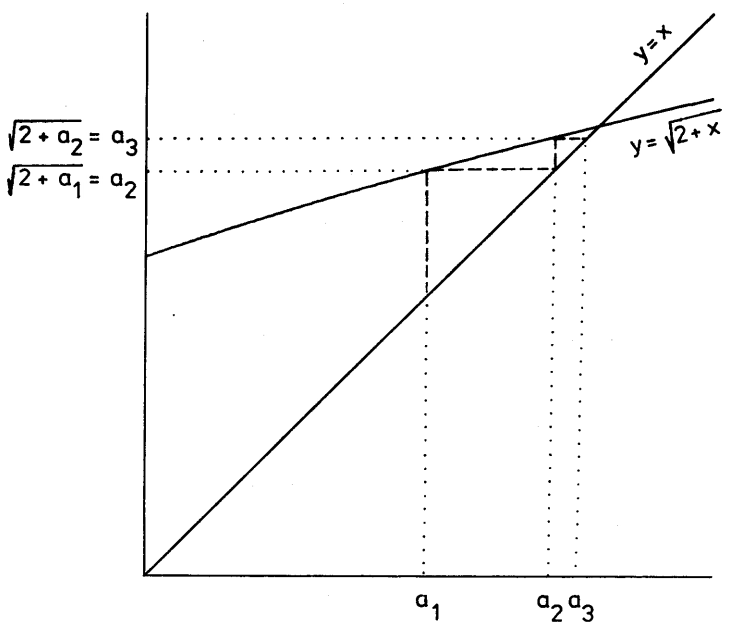
\includegraphics[scale=0.5]{img/pr. 156.png}
\end{center}

    \textit{Poznámka:}
    Rovnosť $\lim\limits_{n \rightarrow \infty} a_n=2$ vyplýva z rovnosti (*),
    mohlo by sa teda zdať, že stačilo len v rekurentnom vzťahu
    $a_{n+1}=\sqrt{2+a_n}$ prejsť k limite a príklad by bol vyriešený, t.j.
    všetky úvahy o monotónnosti a ohraničenosti boli vlastne zbytočné. To je
    ovšem omyl; skôr ako napíšeme (*), sa totiž musíme presvedčiť, že limity,
    ktoré tam vystupujú, skutočne existujú.
\end{solution}
\end{defproblem}

\begin{defproblem}{limita-157}
Dokážte, že postupnosť $a_{n}=(1+\frac{1}{n})^{n+1}$ je klesajúca a zdola
ohraničená. Na základe toho dokážte nerovnosť
\[
    (1+\frac{1}{n})^n<e<(1+\frac{1}{n})^{n+1}
\]
\end{defproblem}

\begin{defproblem}{limita-158}
Dokážte, že neexistujú nasledujúce limity:
\begin{tasks}(3)
    \task $\lim\limits_{{x \rightarrow \infty}} \sin x$
    \task $\lim\limits_{{x \rightarrow a}} \zeta (x), (a \in \mathbb{R^*})$
    \task $\lim\limits_{{x \rightarrow 0}} \cos \frac{\pi}{x}$
    \task! $\lim\limits_{{x \rightarrow -\infty}} f(x)$, ak $f$ je nekonečná periodická funkcia
\end{tasks}

\begin{solution}
    \textbf{a):}
    Pre postupnosti $a_n=n\pi,b_n=\frac{\pi}{2}+2\pi n$ platí
    \[
        a_n = \lim\limits_{n \rightarrow \infty} a_n
            = \lim\limits_{n \rightarrow \infty} b_n
            = \infty
    \]
    \[
        \lim\limits_{n \rightarrow \infty} \sin a_n=0
    \]
    \[
        \lim\limits_{n \rightarrow \infty} b_n=1
    \]
    Pre žiadne $b \in \mathbb{R}^*$ teda nemôže byť splnená
    vlastnosť $2$ z vety $15$, preto neexistuje $\lim\limits_{n \rightarrow \infty}
    \sin x$.
\end{solution}
\end{defproblem}

\begin{defproblem}{limita-159}
Nech $f$ je funkcia definovaná na $\mathbb{R}$, $a \in \mathbb{R^*}$. Rozhodnite, či tvrdenie $\lim\limits_{x \rightarrow a} f(x)=b$ je ekvivalentné s niektorým z nasledujúcich výrokov:
\begin{tasks}
\task pre každú postupnosť ${\{a_n\}}_{n=1}^\infty$ racionálnych čísel takú, že $a_n \neq a$ pre všetky $n \in \mathbb{N}$ a $\lim\limits_{n \rightarrow \infty} a_n=a$, platí $\lim\limits_{n \rightarrow \infty} f(a_n)=b$
\task pre každú postupnosť ${\{a_n\}}_{n=1}^\infty$ takú, že $\lim\limits_{n \rightarrow \infty} a_n=a$, pričom množina $\{ a_n : n\in \mathbb{N }\}$ je podmnožinou $Q \setminus \{ a\}$ alebo podmnožinou $\mathbb{R} \setminus (\mathbb{Q} \cup \{ a\})$ platí $\lim\limits_{n \rightarrow \infty} f(a_n)=b$
\end{tasks}
\end{defproblem}

\begin{defproblem}{limita-160}
Nájdite limes superior a limes inferior nasledujúcich postupností:
\begin{tasks}
    \task $a_n=(-1)^{n-1}(2+\frac{3}{n})$
    \task $a_n=1+2 \cdot (-1)^{n+1}+3 \cdot (-1)^{\frac{n(n-1)}{2}}$
\end{tasks}
\begin{tasks}[resume](2)
    \task $a_n=\cos \frac{n \pi}{3}$
    \task $a_n=(1+\frac{1}{n})^n(-1)^n+\sin \frac{n \pi}{4}$
    \task $a_n=n^{(-1)^n}$
    \task $a_n=\sqrt[n]{1+2^{n \cdot (-1)^n}}$
\end{tasks}
\begin{tasks}[resume]
    \task $1,\frac{1}{10},\frac{2}{10},...,\frac{9}{10},\frac{1}{10^2},\frac{2}{10^2},...,\frac{99}{10^2},...,\frac{1}{10^n},...,\frac{10^n-1}{10^n},...$
    \task $1,\frac{1}{2},\frac{2}{2},\frac{3}{2},\frac{1}{4},\frac{2}{4},...,\frac{5}{4},...,\frac{1}{2^n},...,\frac{2^n+1}{2^n},... $
\end{tasks}
\end{defproblem}

\begin{defproblem}{limita-161}
Zostrojte postupnosť ${\{a_n\}}_{n=1}^\infty$ tak, aby množina jej hromadných
hodnôt bola:
\begin{tasks}(3)
\task $\{ 1\}$
\task $\{ 0,1\}$
\task $\mathbb{N} \cup \{ +\infty \}$
\task* daná konečná množina $\{ a_1,...,a_n\}$
\end{tasks}
\end{defproblem}

\begin{defproblem}{limita-162}
Nech ${\{a_n\}}_{n=1}^\infty$ je postupnosť taká, že $\{ a_n: n \in \mathbb{N}
\}=\mathbb{Q}$ (taká postupnosť existuje, pretože $\mathbb{Q}$ je spočítateľná
množina). Potom množina hromadných hodnôt postupnosti ${\{a_n\}}_{n=1}^\infty$
je $\mathbb{R^*}$. Dokážte!
\end{defproblem}

\begin{defproblem}{limita-163}
Nech ohraničená postupnosť ${\{a_n\}}_{n=1}^\infty$ má práve dve hromadné
hodnoty: označme $a := \liminf\limits_{n \rightarrow \infty} a_n,b :=
\lim\limits_{n \rightarrow \infty} \sup a_n$. Dokážte: pre každé $\varepsilon \in
(0,\frac{b-a}{2})$ je množina $\mathbb{N_\varepsilon} := \{n \in \mathbb{N}; a_n
\in \interval{a + \varepsilon}{b - \varepsilon} \}$ konečná.
\end{defproblem}

\begin{defproblem}{limita-164}
Nech pre ohraničenú postupnosť ${\{a_n\}}_{n=1}^\infty$ platí
\[
    (\forall \varepsilon > 0):
    \lim\limits_{n \rightarrow \infty} \sup a_n
    <
    \lim\limits_{n \rightarrow \infty} \inf a_n+\varepsilon
\]
Potom je postupnosť ${\{a_n\}}_{n=1}^\infty$
konvergentná. Dokážte!
\end{defproblem}

\begin{defproblem}{limita-165}
\begin{tasks}
\task
    Nech $a$ je hromadný bod množiny $A$ hromadných hodnôt postupnosti
    ${\{a_n\}}_{n=1}^\infty$. Potom $a$ je h romadnou hodnotou postupnosti
    ${\{a_n\}}_{n=1}^\infty$.
\task
    Existuje postupnosť, ktorej množina hromadných hodnôt je $A=\{ \frac{1}{n};
    n \in \mathbb{N} \}$ ?
\end{tasks}
\end{defproblem}

\begin{defproblem}{limita-166}
\begin{tasks}
\task
    Nech sú dané ohraničené postupnosti ${\{a_n\}}_{n=1}^\infty$ a
    ${\{b_n\}}_{n=1}^\infty$. Potom:
    \begin{enumerate}[leftmargin=0mm]
    \item ak existuje konečná $\lim\limits_{n \rightarrow \infty} a_n$, tak
        \[
            \lim\limits_{n \rightarrow \infty} \inf (a_n+b_n)=\lim\limits_{n \rightarrow
            \infty} a_n+\lim\limits_{n \rightarrow \infty} \inf b_n
        \]
    \item
        \begin{multline*}
            \lim\limits_{n \rightarrow \infty} \inf a_n + \lim\limits_{n \rightarrow
                \infty} \inf b_n
                \leq \lim\limits_{n \rightarrow \infty} \inf (a_n+b_n) \leq \\
            \leq \lim\limits_{n \rightarrow \infty} \inf a_n
                + \lim\limits_{n \rightarrow \infty} \sup b_n \leq
            \lim\limits_{n \rightarrow \infty} \sup (a_n+b_n) \leq \\
            \leq \lim\limits_{n\rightarrow \infty} \sup a_n+\lim\limits_{n \rightarrow \infty} \sup b_n
        \end{multline*}
    \end{enumerate}
\task
    Uveďte príklady postupností ${\{a_n\}}_{n=1}^\infty$ a
    ${\{b_n\}}_{n=1}^\infty$, pre ktoré budú jednotlivé nerovnosti v príklade
    $166.1b/$ ostré.
\end{tasks}

\begin{solution}
    Dokážeme druhú nerovnosť z príkladu $166.1b/$. (Skôr ako začneme vlastný
    dôkaz, musíme si uvedomiť, že $\lim\limits_{n \rightarrow \infty} \inf
    (a_n+b_n),\lim\limits_{n \rightarrow \infty} \inf a_n, \lim\limits_{n
    \rightarrow \infty} \sup b_n$ sú reálne čísla, pretože postupnosti
    ${\{a_n+b_n\}}_{n=1}^\infty$,${\{a_n\}}_{n=1}^\infty$,${\{b_n\}}_{n=1}^\infty$
    sú ohraničené.) Využijeme nasledujúce nerovnosti: Ak
    ${\{c_{n(k)}\}}_{k=1}^\infty$ je postupnosť vybraná z postupnosti
    $\{c_n\}_{n=1}^\infty$, tak:
    \[
        \lim\limits_{n \rightarrow \infty} \inf c_n
        \leq \lim\limits_{k \rightarrow \infty} \inf c_{n(k)} \leq \lim\limits_{k
        \rightarrow \infty} \sup c_{n(k)}\leq \lim\limits_{k \rightarrow \infty}
        \sup c_n
    \]
    (nerovnosť $(2)$ je zrejmé, nerovnosti $(1)$ a $(3)$ vyplývajú z
    faktu, že každá hromadná hodnota postupnosti ${\{c_{n(k)}\}}_{k=1}^\infty$
    je aj hodnotou postupnosti ${\{c_n\}}_{n=1}^\infty$, t.j. že množina
    hromadných hodnôt postupnosti ${\{c_{n(k)}\}}_{k=1}^\infty$ je podmnožina
    množiny hromadných hodnôt postupnosti ${\{c_n\}}_{n=1}^\infty$).

    Nech $a:=\lim\limits_{n \rightarrow \infty} a_n$, potom existuje postupnosť
    ${\{a_n\}}_{n=1}^\infty$ taká, že $\lim\limits_{k \rightarrow \infty}
    a_{n(k)}=a=\lim\limits_{n \rightarrow \infty} \inf a_n$. Podľa príkladu
    $166.1a)$ je:
    \[
        \lim\limits_{k \rightarrow \infty} \inf (a_{n(k)}+b_{n(k)}) =
        \lim\limits_{k \rightarrow \infty} a_{n(k)}+\lim\limits_{k \rightarrow
        \infty}
        \inf b_{n(k)}
    \]
    \[
        (=\lim\limits_{n \rightarrow \infty}
        \inf a_n + \lim\limits_{n \rightarrow \infty} \inf b{n(k)})
    \]
    Na dokončenie dôkazu teraz už stačí len niekoľkokrát použiť nerovnosti z
    (*):
    \[
        \lim\limits_{n \rightarrow \infty} \inf (a_n+b_n)
        \leq \lim\limits_{k \rightarrow \infty} \inf (a_{n(k)}+b_{n(k)})
        =
    \]
    \[
        = \lim\limits_{\rightarrow \infty} \inf a_n
            + \lim\limits_{n \rightarrow \infty} \inf b_{n(k)}
            \leq \lim\limits_{n \rightarrow \infty} \inf a_n
            + \lim\limits_{k \rightarrow \infty} \sup b_{n(k)}
        \leq
    \]
    \[
        \leq \lim\limits_{n \rightarrow \infty} \inf a_n
            +\lim\limits_{n \rightarrow \infty} \sup b_n
    \]
    (ak zapíšeme nerovnosť $(1)$ z (*) pre postupnosti:
    \[ c_n=a_n+b_n,c_{n(k)}=a_{n(k)}+b_{n(k)} \]
    dostaneme (I); nerovnosť (II) dostaneme, ak k obidvom stranám nerovnosti
    $(2)$ z (*) zapísanej pre postupnosť ${\{b_{n(k)}\}}_{k=1}^\infty$
    pripočítame číslo $\lim\limits_{\rightarrow \infty} \inf a_n$, podobne
    vyplýva (III) z nerovnosti $(3)$ v (*)).
\end{solution}
\end{defproblem}

\begin{defproblem}{limita-167}
Uveďte príklad neprázdnej množiny $a \subset \mathbb{R}$, že $A' \neq \emptyset$
a platí
\begin{tasks}(4)
\task $A' \subsetneq A$
\task $A'=A$
\task $A \subsetneq A'$
\task $A' \cap A = \emptyset$
\task! $A \not\subset A'\wedge A' \not\subset A \wedge A' \cap A \neq\emptyset$
\end{tasks}
\end{defproblem}

\begin{defproblem}{limita-168}
Ak $a \in \mathbb{R^*}$ je hromadný bod množiny $A'$, tak $a$ je aj hromadný bod
množiny $A$ (teda $(A')' \subset A'$). Dokážte!
\end{defproblem}

\begin{defproblem}{limita-169}
Existuje množiny $A$ taká, že $A'=(0,1)$?
\end{defproblem}

\begin{defproblem}{limita-170}
Nech $a \in \mathbb{R^*}$ je hromadný bod množiny $A \cup B$. Potom $a$ je
hromadný bod množiny $A$ alebo $a$ je hromadný bod množiny $B$ (teda $(A \cup
B)' \subset A' \cup B'$). Dokážte!
\end{defproblem}

\begin{defproblem}{limita-171}
Nech je daná postupnosť ${\{a_n\}}_{n=1}^\infty$, definujme postupnosť
${\{b_n\}}_{n=1}^\infty$ predpisom
\[b_n=\frac{1}{n}(a_1+a_2+...+a_n)\]
Ak $\lim\limits_{n \rightarrow \infty} a_n=a (a \in \mathbb{R^*})$, tak existuje
aj $\lim\limits_{n \rightarrow \infty} b_n$ a platí $\lim\limits_{n \rightarrow
\infty} a_n=a$. Dokážte; ďalej ukážte, že obrátená implikácia vo všeobecnosti
neplatí.
\end{defproblem}

\begin{defproblem}{limita-172}
Nájdite limity:
\begin{tasks}(2)
\task $\lim\limits_{n \rightarrow \infty} \frac{1}{n}(1+\frac{1}{2}+...+\frac{1}{n})$
\task $\lim\limits_{n \rightarrow \infty} \frac{1}{n}(1+\frac{1}{\sqrt{2}}+...+\frac{1}{\sqrt{n}})$
\end{tasks}
\end{defproblem}

\begin{defproblem}{limita-173}
\begin{tasks}
\task
    Nech ${\{a_n\}}_{n=1}^\infty$ je postupnosť taká, že $\{ a_n: n \in
    \mathbb{N} \}=\mathbb{N}$. Potom existuje $\lim\limits_{n \rightarrow
    \infty} a_n$ a rovná sa $+\infty$.
\task
    Postupnosť ${\{b_n\}}_{n=1}^\infty$ sa nazýva prerovnaním postupnosti
    ${\{a_n\}}_{n=1}^\infty$, ak existuje taká bijekcia $p: \mathbb{N}
    \rightarrow \mathbb{N}$, že
    \[
        b_n=a_{p(n)},(n \in \mathbb{N})
    \]
    Ak $\lim\limits_{n \rightarrow \infty} a_n=b,(b \in \mathbb{R^*})$, tak každé
    prerovnanie postupnosti ${\{a_n\}}_{n=1}^\infty$, má tiež limitu rovnú $b$.
    Dokážte!
\end{tasks}
\end{defproblem}

\begin{defproblem}{limita-174}
Zostane tvrdenie z príkladu $173.(a)$  v platnosti, ak v ňom
\begin{tasks}
\task vynecháme predpoklad "${\{a_n\}}_{n=1}^\infty$, je prostá postupnosť"?
\task Predpoklad "$\{a_n: n \in \mathbb{N}\}=\mathbb{N}$" nahradíme predpokladom "$\{a_n: n \in \mathbb{N}\} \subset \mathbb{N}$"?
\end{tasks}
\end{defproblem}

\begin{defproblem}{limita-175}
Nech ${\{a_n\}}_{n=1}^\infty$ je taká postupnosť, že existuje $\lim\limits_{n \rightarrow \infty} |a_n|=b$ a neexistuje $\lim\limits_{n \rightarrow \infty} a_n$. Dokážte, že
\begin{tasks}
\task $b \neq 0$
\task množiny $\mathbb{N^+}:= \{n \in \mathbb{N}: a_n>0 \}$ a $\mathbb{N^-}:= \{n \in \mathbb{N}: a_n<0 \}$ sú konečné
\task množina $\mathbb{N} \setminus (\mathbb{N^+} \cup \mathbb{N^-})$ je konečná
\end{tasks}
\end{defproblem}

\begin{defproblem}{limita-176}
Na základe definície limity dokážte:
\begin{tasks}(2)
    \task $\lim\limits_{n \rightarrow \infty} \frac{5 \cdot 3^n}{3^n-2}=5$
    \task $\lim\limits_{x \rightarrow \infty} \arccot x=\frac{\pi}{2}$
\end{tasks}
\end{defproblem}

\begin{defproblem}{limita-177}
Uveďte príklad funkcie $f: \mathbb{R} \rightarrow \mathbb{R}$, Ktorá má limitu len v bode $0$.
\end{defproblem}

\begin{defproblem}{limita-178}
Dokážte, že postupnosť ${\{\sin n\}}_{n=1}^\infty$ nemá limitu.
\end{defproblem}

\begin{defproblem}{limita-179}
Nájdite limity:
\begin{tasks}(2)
    \task* $\lim\limits_{x \rightarrow 0} \frac{(1+mx)^n-(1+nx)^m}{x^2},(m,n \in \mathbb{N})$
    \task $\lim\limits_{x \rightarrow a} \frac{x^n-a^n-na^{n-1}(x-a)}{(x-a)^2}$
    \task $\lim\limits_{x \rightarrow 1} (\frac{3}{1-x^2}-\frac{1}{x-1})$
    \task* $\lim\limits_{x \rightarrow 1} (\frac{m}{1-x^m}-\frac{n}{1-x^n}),(m,n \in \mathbb{N})$
    \task* $\lim\limits_{x \rightarrow \infty} \frac{1}{n}[(x+\frac{a}{n})^2+(x+\frac{2a}{n})^2+...+(x+\frac{n-1}{n}a)^2]$
    \task $\lim\limits_{n\rightarrow \infty} \frac{(x+1)(x^2+1)...(x^n+1)}{[(nx)^n+1]^{\frac{n+1}{2}}}$
    \task $\lim\limits_{n \rightarrow \infty} \frac{(n+4)!-(n+2)!}{(n+3)!}$
    \task $\lim\limits_{n \rightarrow \infty} \frac{1+3+...+(2n-1)}{1+4+...+(3n-2)}$
    \task $\lim\limits_{n \rightarrow \infty} \frac{1-2+3-4+...+(-1)^{n-1}n}{n}$
    \task $\lim\limits_{x \rightarrow \infty} (\frac{5}{6}+\frac{13}{36}+...+\frac{2^n-3^n}{6^n})$
\end{tasks}
\end{defproblem}

\begin{defproblem}{limita-180}
Nech ${\{a_n\}}_{n=1}^\infty$ je konvergentná postupnosť. Potom existuje maximum alebo minimum množiny $\{a_n: n \in \mathbb{N}\}$. Dokážte!
\end{defproblem}

\begin{defproblem}{limita-181}
Dokážte, že neexistuje racionálna funkcia $\mathbb{R}$ s celočíselnými
koeficientami taká, aby platilo
\[
    (\forall r \in \mathbb{Q})
        (\exists k \in \mathbb{Z}):
            R(k)=r
\]
\end{defproblem}

\begin{defproblem}{limita-182}
Nájdite limity:
\begin{tasks}
\task $\lim\limits_{x \rightarrow 0} \frac{\sqrt[m]{1+\alpha x}-\sqrt[n]{1+\beta x}}{x},(m,n \in \mathbb{Z})$
\task $\lim\limits_{x \rightarrow 0}  \frac{\sqrt[m]{1+\alpha x}\sqrt[n]{1+\beta x}-1}{x},(m,n \in \mathbb{Z})$
\task $\lim\limits_{x \rightarrow 0} (\sqrt{\frac{1}{x}+\sqrt{\frac{1}{x}+\sqrt{\frac{1}{x}}}}-\sqrt{\frac{1}{x}+\sqrt{\frac{1}{x}+\sqrt{\frac{1}{x}}}})$
\task $\lim\limits_{x \rightarrow -\infty} (x+\sqrt{\frac{x^3+2x^2}{x+1}})$
\task $\lim\limits_{x \rightarrow -\infty} \arcsin (\sqrt{x^2+x}+x)$
\task $\lim\limits_{x \rightarrow \infty} \frac{\sqrt{3x-1}-\sqrt[3]{125n^3+n}}{\sqrt[5]{n}-n}$
\task $\lim\limits_{x \rightarrow \infty} x^{\frac{3}{2}}(\sqrt{x+2}-2\sqrt{x+1}+\sqrt{x})$
\task $\lim\limits_{x \rightarrow \infty} (\sqrt[3]{x^3+3x^2}-\sqrt{x^2-2x})$
\task $\lim\limits_{x \rightarrow \infty} \frac{(x-\sqrt{x^2-1})^n+(x+\sqrt{x^2-1})^n}{x^n}, (n \in \mathbb{N})$
\end{tasks}
\end{defproblem}

\begin{defproblem}{limita-183}
Nech $f,g: \mathbb{R} \rightarrow \mathbb{R}$ sú periodické funkcie a $\lim\limits_{x \rightarrow \infty} (f(x)-g(x)=0)$. Potom $f=g$. Dokážte!
\end{defproblem}

\begin{defproblem}{limita-184}
\begin{tasks}(2)
    \task $\lim\limits_{x \rightarrow 0} \frac{\cos 3x^3-1}{\sin ^6 2x}$
    \task $\lim\limits_{x \rightarrow 0} \frac{\sin (a+2x)-2\sin (a+x)+\sin a}{x^2}$
    \task $\lim\limits_{x \rightarrow 0} \frac{4\sin (\frac{\pi}{6}+x)\sin (\frac{\pi}{6}+2x)-1}{\sin x}$

    \task $\lim\limits_{x \rightarrow 2} \frac{\arctan (x^2-2x)}{\sin 3\pi x}$
    \task $\lim\limits_{x \rightarrow 0} \frac{\arctan \frac{1}{x}+2}{x^2}$
    \task $\lim\limits_{x \rightarrow 0} \frac{1-\cos x\sqrt{\cos 2x}\sqrt[3]{\cos 3x}}{x^2}$
    \task $\lim\limits_{x \rightarrow \frac{\pi}{3}} \frac{\tan^3 x-3 \tan c}{\cos (x+\frac{\pi}{6})}$
    \task $\lim\limits_{x \rightarrow 0} \frac{\arcsin (1-x)}{\sqrt{x}}$
    \task $\lim\limits_{x \rightarrow \frac{1}{2}} \frac{\arccos x}{(2x-1)^2}$
    \task $\lim\limits_{x \rightarrow \frac{\pi}{2}} \frac{1-\sin ^3 x}{\cos ^2 x}$
    \task $\lim\limits_{x \rightarrow 1} \frac{\sqrt{\sin \frac{\pi x}{2}}+\sqrt[3]{\sin \frac{3\pi x}{2}}}{\sqrt{x^2+1}-\sqrt{2x}}$
    \task $\lim\limits_{x \rightarrow 1} \frac{\cos \frac{\pi x}{2}}{x-1}\cdot \frac{\sqrt{x+3}-2}{\sqrt{x^3+3x}-\sqrt{3x^2+1}}$
    \task $\lim\limits_{x \rightarrow 0} \frac{1-\sqrt{\cos x}}{1-\cos \sqrt{x}}$
    \task $\lim\limits_{x \rightarrow \frac{\pi}{2}} \sqrt{\frac{(2x-\pi)\sin \frac{\pi}{2x-\pi}}{\cos 4x}}$
    \task $\lim\limits_{x \rightarrow \infty} (\sin \ln (x+1)-\sin \ln x)$
\end{tasks}
\end{defproblem}

\begin{defproblem}{limita-185}
\begin{tasks}
\task Nech $q \in (0,1)$, nech pre postupnosť ${\{a_n\}}_{n=1}^\infty$ nezáporných čísel platí $\sqrt[n]{a_n}\leq q,(n \in \mathbb{N})$. Potom $\lim\limits_{n \rightarrow \infty} a_n=0$. Dokážte!
\task Nájdite $\lim\limits_{n \rightarrow \infty}\frac{n^{n-1}}{(2n^2+n+1)^{\frac{n+1}{2}}}$.
\end{tasks}
\end{defproblem}

\begin{defproblem}{limita-186}
Dokážte, že
\begin{tasks}(2)
\task $\lim\limits_{n \rightarrow \infty} \frac{n^k}{a^n}=0,(k \in \mathbb{R},a>1)$
\task $\lim\limits_{n \rightarrow \infty} \frac{a^n}{n!}=0$
\task $\lim\limits_{n \rightarrow \infty} \frac{1}{\sqrt[n]{n!}}=0$
\end{tasks}
\end{defproblem}

\begin{defproblem}{limita-187}
\begin{tasks}(2)
    \task $\lim\limits_{n \rightarrow \infty} \sqrt[n]{\frac{2n^2-5n+3}{n^5+1}}$
    \task $\lim\limits_{n \rightarrow \infty} \sqrt[n]{a^n+b^n},(a,b>0)$
    \task $\lim\limits_{n \rightarrow \infty} \sqrt[n]{3^n+n2^n}$
    \task $\lim\limits_{n \rightarrow \infty} (1+11^n)^{\frac{1}{n+2}}$
    \task $\lim\limits_{n \rightarrow \frac{\pi}{2}} \frac{2^nn!}{n^n}$
    \task $\lim\limits_{n \rightarrow \infty} \frac{3^nn!}{n^n}$
    \task $\lim\limits_{n \rightarrow \infty} \frac{n!}{4^n}$
    \task $\lim\limits_{n \rightarrow \infty} \frac{n^3+3^n}{n+3^{n+1}}$
    \task $\lim\limits_{n \rightarrow \infty} \frac{2^{\frac{n}{2}}+(n+1)!}{n(3^n+n!)}$
    \task $\lim\limits_{n \rightarrow \infty} \frac{2}{1-\sqrt[n]{n}}$
\end{tasks}
\end{defproblem}

\begin{defproblem}{limita-188}
Nech $x_n=\sum_{k=1}^n \frac{1}{\sqrt{n^2+k}}$; ukážeme dva spôsoby výpočtu $\lim\limits_{n \rightarrow \infty} x_n:$
\begin{tasks}
\task odhadneme $x_n$ zhora a zdola:
\[
    x_n=\sum_{k=1}^n \frac{1}{\sqrt{n^2+n}}
    \leq
    \sum_{k=1}^n \frac{1}{\sqrt{n^2+k}}
    \leq
    \sum_{k=1}^n \frac{1}{\sqrt{n^2}}=1
\]
teda
\[
    \frac{n}{\sqrt{n^2+n}}\leq x_n \leq 1, (n \in \mathbb{N})
\]
Pretože $\lim\limits_{n \rightarrow \infty}
\frac{n}{\sqrt{n^2+n}}=1=\lim\limits_{n \rightarrow \infty} 1$, je podľa vety
$6$ $\lim\limits_{n \rightarrow \infty} x_n=1$. \task Podľa vety o limite súčtu
je
\begin{multline*}
    \lim\limits_{n \rightarrow \infty} \sum_{k=1}^n
        \frac{1}{\sqrt{n^2+k}}
        =\lim\limits_{n \rightarrow \infty}
        \frac{n}{\sqrt{n^2+1}}+\lim\limits_{n \rightarrow \infty}
        \frac{n}{\sqrt{n^2+2}} + \\
        + ... + \lim\limits_{n \rightarrow \infty}
        \frac{n}{\sqrt{n^2+n}}
        = 0 + 0 + ... + 0 = 0
\end{multline*}
Zrejme aspoň jeden z uvedených postupov je nesprávny. Ktorý to je a v čom
spočíva chyba?
\end{tasks}
\end{defproblem}

\begin{defproblem}{limita-189}
Sformulujte a dokážte pravidlá pre výpočet limít typu $0^{+\infty}$ a
$0^{-\infty}$.
\end{defproblem}

\begin{defproblem}{limita-190}
Nájdite limity:
\begin{tasks}(2)
    \task $\lim\limits_{n \rightarrow \infty} (\frac{3x^2-x+1}{2x^2+x+1})^{\frac{x^3}{1-x}}$
    \task $\lim\limits_{n \rightarrow \infty} \tan ^n (\frac{\pi}{4}+\frac{1}{n})$
    \task $\lim\limits_{n \rightarrow \infty} (\frac{2^x}{1+x^{x+1}})^{-x^2}$
    \task $\lim\limits_{n \rightarrow 0} \sqrt[x]{\cos \sqrt{x}}$
    \task $\lim\limits_{n \rightarrow 0} (1-\cos x)^{\frac{1}{x^2}}$
    \task $\lim\limits_{n \rightarrow \frac{\pi}{4}} (\tan (\frac{\pi}{8}+x))^{\tan 2x}$
    \task $\lim\limits_{n \rightarrow 0} (\frac{1+\sin x \cos ^ \alpha x}{1+\sin x \cos \beta x})^{\coth ^3 x}$
    \task $\lim\limits_{n \rightarrow \frac{\pi}{3}} (\cos x)^{\frac{1}{(3x-\pi)^3}}$
    \task $\lim\limits_{n \rightarrow \infty} (\frac{a_1x+b_1}{a_2x+b_2})^x,(a_1,a_2>0)$
    \task $\lim\limits_{n \rightarrow 1} (\frac{\sin (x-1)}{x-1})^{\frac{\sin (x-1)}{x-1-\sin (x-1)}}$
    \task $\lim\limits_{n \rightarrow \infty} \frac{(x+a)^{x+a}(x+b)^{x+b}}{(x+a+b)^{2x+a+b}}$
\end{tasks}
\end{defproblem}

\begin{defproblem}{limita-191}
Nájdite limity:
\begin{tasks}(2)
    \task $\lim\limits_{n \rightarrow 1} (1-x)\log_x 2$
    \task $\lim\limits_{n \rightarrow \infty} \ln (1+2^x) \ln (1+\frac{3}{x})$
    \task $\lim\limits_{n \rightarrow \infty} \ln \frac{x+\sqrt{x^2+1}}{x+\sqrt{x^2-1}} \cdot \ln ^{-2} \frac{x+1}{x-1}$
    \task $\lim\limits_{n \rightarrow a} \frac{x^\alpha-a^\alpha}{x-a},(a>0,\alpha \in \mathbb{R})$
    \task $\lim\limits_{n \rightarrow a} \frac{x^x-a^a}{x-a},(a>0)$
    \task $\lim\limits_{n \rightarrow \infty} (\frac{\sqrt[n]{a}+\sqrt[n]{b}}{2})^n,(a.b>0)$
    \task $\lim\limits_{n \rightarrow \infty} n^2(\sqrt[n]{x}-\sqrt[n+1]{x}),(x>0)$
    \task $\lim\limits_{n \rightarrow 0} \frac{a^{x^2}-b^{x^2}}{(a^x-b^x)^2},(a,b>0)$
    \task $\lim\limits_{n \rightarrow 0} (\frac{a^{x^2}-b^{x^2}}{(a^x-b^x)^2})^{\frac{1}{x}},(a,b>0)$
    \task $\lim\limits_{n \rightarrow 0} \frac{\cos (xe^x)-\cos (xe^{-x})}{x^3}$
    \task $\lim\limits_{n \rightarrow 1} \frac{\sin ^2 \pi x^\alpha}{\sin ^2 \pi x^\beta},(\beta \neq 0)$
    \task $\lim\limits_{n \rightarrow 1} \frac{\sin ^2 \pi 2^{x}}{\ln (\cos \pi 2^{x})}$
\end{tasks}
\end{defproblem}

\begin{defproblem}{limita-192}
\begin{tasks}
\task Dokážte pre $a > 1,\alpha > 0$, že:
    \begin{enumerate*}
        \item $\lim\limits_{n \rightarrow \infty} \frac{x^{\alpha}}{a^x}=0$
        \item $\lim\limits_{x \rightarrow \infty} \frac{\log_a x}{x^\alpha}=0$
    \end{enumerate*}
\task Nájdite:
    \begin{enumerate*}
        \item $\lim\limits_{n \rightarrow 0} x^{\frac{1}{100}^{-\frac{1}{x^2}}}$
        \item $\lim\limits_{x \rightarrow 0} x \ln x$
        \item $\lim\limits_{x \rightarrow \infty} (\frac{1}{n})^{\tan \frac{1}{n}}$
    \end{enumerate*}
\end{tasks}
\textit{Poznámka:}
Tvrdenie z príkladu $192.(a)$ si možno zapamätať v nasledujúcej symbolickej
podobe $\log_a x\ll x^\alpha \ll a^x$ (pre $x$ dostatočne veľké, $\alpha >0,
a>0$) kde $f\ll g$ (pre dostatočne veľké x) znamená $\lim\limits_{x \rightarrow
\infty} \frac{f(x)}{g(x)}=0$. Pre postupnosti platí (pozri aj príklad $186$):
$\log_a n\ll n^\alpha\ll a^n\ll n!$ (pre $n$ dostatočne veľké,  $\alpha >0,
a>0$)
\end{defproblem}

\begin{defproblem}{limita-193}
Nech $\lim\limits_{x \rightarrow a} \frac{\alpha (x)}{\alpha_1 (x)}$ a
$\lim\limits_{x \rightarrow a} \frac{\beta (x)}{\beta_1(x)}$ sú konečné a
nenulové. Potom $\lim\limits_{x \rightarrow a} \frac{\alpha (x)}{\beta (x)}$
existuje práve vtedy, keď existuje $\lim\limits_{x \rightarrow a} \frac{\alpha_1
(x)}{\beta_1 (x)}$. Dokážte!
\end{defproblem}

\begin{defproblem}{limita-194}
Nech $a$ je definovaná na $\mathbb{R}$ a $\lim\limits_{x \rightarrow 0}
f(x)=+\infty$. Zostrojte funkciu $g: \mathbb{R} \rightarrow \mathbb{R}$, pre
ktorú existuje nenulová $\lim\limits_{x \rightarrow 0} g(x)$ a neexistuje
$\lim\limits_{x \rightarrow 0} \frac{f(x)}{g(x)}$.
\end{defproblem}

\begin{defproblem}{limita-195}
Dokážte, že nasledujúce postupnosti sú konvergentné:
\begin{tasks}
\task $a_n=\frac{(2n)!!}{(2n+1)!!}$, kde $(2n)!!=2\cdot4\cdot...\cdot2n,(2n+1)!!=1\cdot3\cdot...\cdot(2n+1)$
\task $a_n=1+\frac{1}{2^2}+\frac{1}{3^2}+...+\frac{1}{n^2}$
\task $a_n=(1+\frac{1}{2})\cdot(1+\frac{1}{4})\cdot...\cdot(1+\frac{1}{2^n})$
\end{tasks}
\end{defproblem}

\begin{defproblem}{limita-196}
Nech $b_1=1,b_n=\sqrt{1+\sqrt{2+...+\sqrt{n}}}$. Potom ${\{b_n\}}_{n=1}^\infty$ je konvergentná postupnosť. Dokážte!
\end{defproblem}

\begin{defproblem}{limita-197}
Nájdite $\lim\limits_{n \rightarrow \infty} a_n$, ak
\begin{tasks}(2)
    \task $a_1=0,a_2=1,a_{n+2}=\frac{a_n+a_{n+1}}{2}$
    \task $a_1=a,a_2=b,a_{n+2}=\frac{a_n+a_{n+1}}{2}$
\end{tasks}
\end{defproblem}

\begin{defproblem}{limita-198}
Nech $f$ je funkcia definovaná na $\mathbb{R}$, $a \in \mathbb{R^*},b \in
\mathbb{R^*}$. Rozhodnite, či tvrdenie $\lim\limits_{x \rightarrow f(x)=b}$ je
ekvivalentné s niektorým z nasledujúcich výrokov:
\begin{tasks}
\task
    pre každú monotónnu postupnosť ${\{a_n\}}_{n=1}^\infty$ takú, že
    $\lim\limits_{x \rightarrow \infty} a_n=a$, pričom $a_n \neq a,(n \in
    \mathbb{N})$ platí $\lim\limits_{x \rightarrow \infty} f(a_n)=b$
\task
    z každej postupnosti ${\{a_n\}}_{n=1}^\infty$, ktorej limitou je $a$, pričom
    $a_n \neq a ,(n \in \mathbb{N})$, možno vybrať postupnosť
    ${\{a_{n(k)}\}}_{n=1}^\infty$ takú, že $\lim\limits_{x \rightarrow \infty}
    f(a_{n(k)})=b$
\end{tasks}
\end{defproblem}

\begin{defproblem}{limita-199}
Nech $a$ je hromadný bod definičného oboru $D(f)$ funkcie $f$. Dokážte, že
nasledujúce dve podmienky sú ekvivalentné:
\begin{tasks}
\task
    neexistuje $\lim\limits_{x \rightarrow \infty} f(x)=b$
\task
    existujú postupnosti ${\{a_n\}}_{n=1}^\infty$, ${\{b_n\}}_{n=1}^\infty$
    prvkov z $D(f) \setminus \{a \}$ také, že $\lim\limits_{n \rightarrow
    \infty} a_n=lim_{n \rightarrow \infty} b_n=a$, $\lim\limits_{x \rightarrow
    \infty} f(a_n)$ a $\lim\limits_{x \rightarrow \infty} f(b_n)$ existujú a
    nerovnajú sa
\end{tasks}
\end{defproblem}

\begin{defproblem}{limita-200}
Nech je daná ohraničená postupnosť ${\{a_n\}}_{n=1}^\infty$. Dokážte, že
\begin{tasks}
    \task
        $\lim\limits_{n \rightarrow \infty}
            \sup a_n=\inf \{\sup\limits_{k \geq n} a_k: n \in \mathbb{N}\}$
    \task
        $\lim\limits_{n \rightarrow \infty}
            \inf a_n= \sup \{\inf\limits_{k \geq n} a_k: n \in \mathbb{N}\}$
\end{tasks}
\end{defproblem}

\begin{defproblem}{limita-201}
Existuje postupnosť taká, že množina jej hromadných hodnôt je
\begin{tasks}(2)
\task $\interval{0}{1}$
\task $\interval[open]{0}{1}$
\end{tasks}
\end{defproblem}

\begin{defproblem}{limita-202}
Nech ${\{a_n\}}_{n=1}^\infty$ je ohraničená postupnosť a $\lim\limits_{n
\rightarrow \infty} (a_{n+1}-a_n)=0$. Dokážte, že množina $H$ hromadných hodnôt
postupnosti ${\{a_n\}}_{n=1}^\infty$ je množina:
\[
    \{x \in \mathbb{R}:
    \lim\limits_{n \rightarrow \infty} \inf a_n \leq x \leq \lim\limits_{n
    \rightarrow \infty} \sup a_n\}
\]
\end{defproblem}

\begin{defproblem}{limita-203}
Nech v postupnosti ${\{a_n\}}_{n=1}^\infty$ konvergujú podpostupnosti
${\{a_{2k}\}}_{k=1}^\infty$, ${\{a_{2k-1}\}}_{k=1}^\infty$,
${\{a_{3k}\}}_{k=1}^\infty$. Dokážte, že potom konverguje aj postupnosť
${\{a_n\}}_{n=1}^\infty$.
\end{defproblem}

\begin{defproblem}{limita-204}
Aké postupnosti vyhovujú podmienke
\begin{tasks}
\task
    $
        (\forall \varepsilon >0)
            (\forall n_0 \in \mathbb{N})
                (\exists n \in \mathbb{N})
                    (n > n_0): |a_n|< \varepsilon
    $
\task
    $
        (\forall \varepsilon > 0)
            (\exists n_0 \in \mathbb{N})
                (\exists n \in \mathbb{N})
                    (n > n_0): |a_n|< \varepsilon
    $
\end{tasks}
\end{defproblem}

\begin{defproblem}{limita-205}
\begin{tasks}
\task
    Nech pre postupnosť ${\{a_n\}}_{n=1}^\infty$ kladných čísel platí
    \[
        \lim\limits_{n \rightarrow \infty} \sup a_n
        \cdot
        \lim\limits_{n \rightarrow \infty} \sup \frac{1}{a_n} = 1
    \]
    Potom ${\{a_n\}}_{n=1}^\infty$ je konvergentná postupnosť. Dokážte!
\task
    Pre ktoré postupnosti ${\{a_n\}}_{n=1}^\infty$ kladných čísel platí vzťah
    \[
        \lim\limits_{n \rightarrow \infty} \inf a_n
        \cdot
        \lim\limits_{n \rightarrow \infty} \sup \frac{1}{a_n}=1
    \]
\end{tasks}
\end{defproblem}

\begin{defproblem}{limita-206}
Nech ${\{a_n\}}_{n=1}^\infty$, ${\{b_n\}}_{n=1}^\infty$ sú ohraničené
postupnosti nezáporných čísel. Dokážte nasledujúce tvrdenia:
\begin{tasks}
\task
    ak existuje konečná $\lim\limits_{n \rightarrow \infty} a_n$, tak:
    \[
        \lim\limits_{n \rightarrow \infty} \inf a_n \cdot b_n
        =\lim\limits_{n \rightarrow \infty} a_n \cdot \lim\limits_{n \rightarrow \infty} \sup b_n
    \]
\task
    \[
        \lim\limits_{n \rightarrow \infty} \inf a_n \cdot \lim\limits_{n \rightarrow
            \infty} \inf b_n
        \leq \lim\limits_{n \rightarrow \infty} \inf a_n \cdot b_n
        \leq
    \]
    \[
        \leq \lim\limits_{n \rightarrow \infty} \inf a_n \cdot \lim\limits_{n \rightarrow
            \infty} \sup b_n
        \leq \lim\limits_{n \rightarrow \infty} \sup a_n \cdot b_n
        \leq
    \]
    \[
        \leq \lim\limits_{n \rightarrow \infty} \sup a_n \cdot \lim\limits_{n \rightarrow
            \infty} \sup b_n
    \]
\end{tasks}
\end{defproblem}

\begin{defproblem}{limita-207}
Nech ${\{a_n\}}_{n=1}^\infty$ je postupnosť kladných čísel, nech
$\lim\limits_{n \rightarrow \infty} \inf a_n =0$. Dokážte, že existuje nekonečne
veľa indexov $n$ takých, že platí
\[
    (\forall k \in \mathbb{N}): k<n \Rightarrow a_k > a_n
\]
(t.j. $a_n$ je menšie než všetky predchádzajúce členy postupnosti
${\{a_n\}}_{n=1}^\infty$).
\end{defproblem}